\chapter{APP AS A DATA ANALYSIS TOOL}
\label{chap:analysis_tool}

\textbf{Data analysis} is a procedure used to examine, clean, change and rebuild information with a view to reach to a specific decision for a given circumstance. Information investigation is normally of two sorts: subjective or quantitative. The sort of information directs the technique for examination. In subjective research, any non-numerical information like content or individual words are broke down. Quantitative examination, then again, centers around estimation of the information and can utilize insights to help uncover results and ends. The outcomes are numerical. At times, the two types of examination are utilized as an inseparable unit. For instance, quantitative investigation can help demonstrate subjective ends. \\

Spatial information investigation is concerned about that part of information examination where the land referencing of articles contains imperative data. This chapter talks about the ways this app can be used as an analysis tool directly or indirectly. \\

\section{Data downloading}

\textbf{Downloading} is defined as the transfer of data from server to your system or belonging. In other words, it is defined as the transmission of data from one machine to another. The significant advantage of downloading is that it gives you the full power over the information with the goal that you can utilize that information. \\

The app gives you the feature of exporting any admim level (0, 1 or 2) data in \gls{csv} format via email option so that it can be used in any form of spatial analysis.

Process of data downloading is described below.

\begin{itemize}
    \item Select year, date and tap on country to see the data and then tap on any region. Once you do that, you will see two buttons on both top corners of the screen. Figure 5.1 shows the two buttons which appears after having valid data on globe / map. \\
    
      \begin{figure}[H]
            \centering
            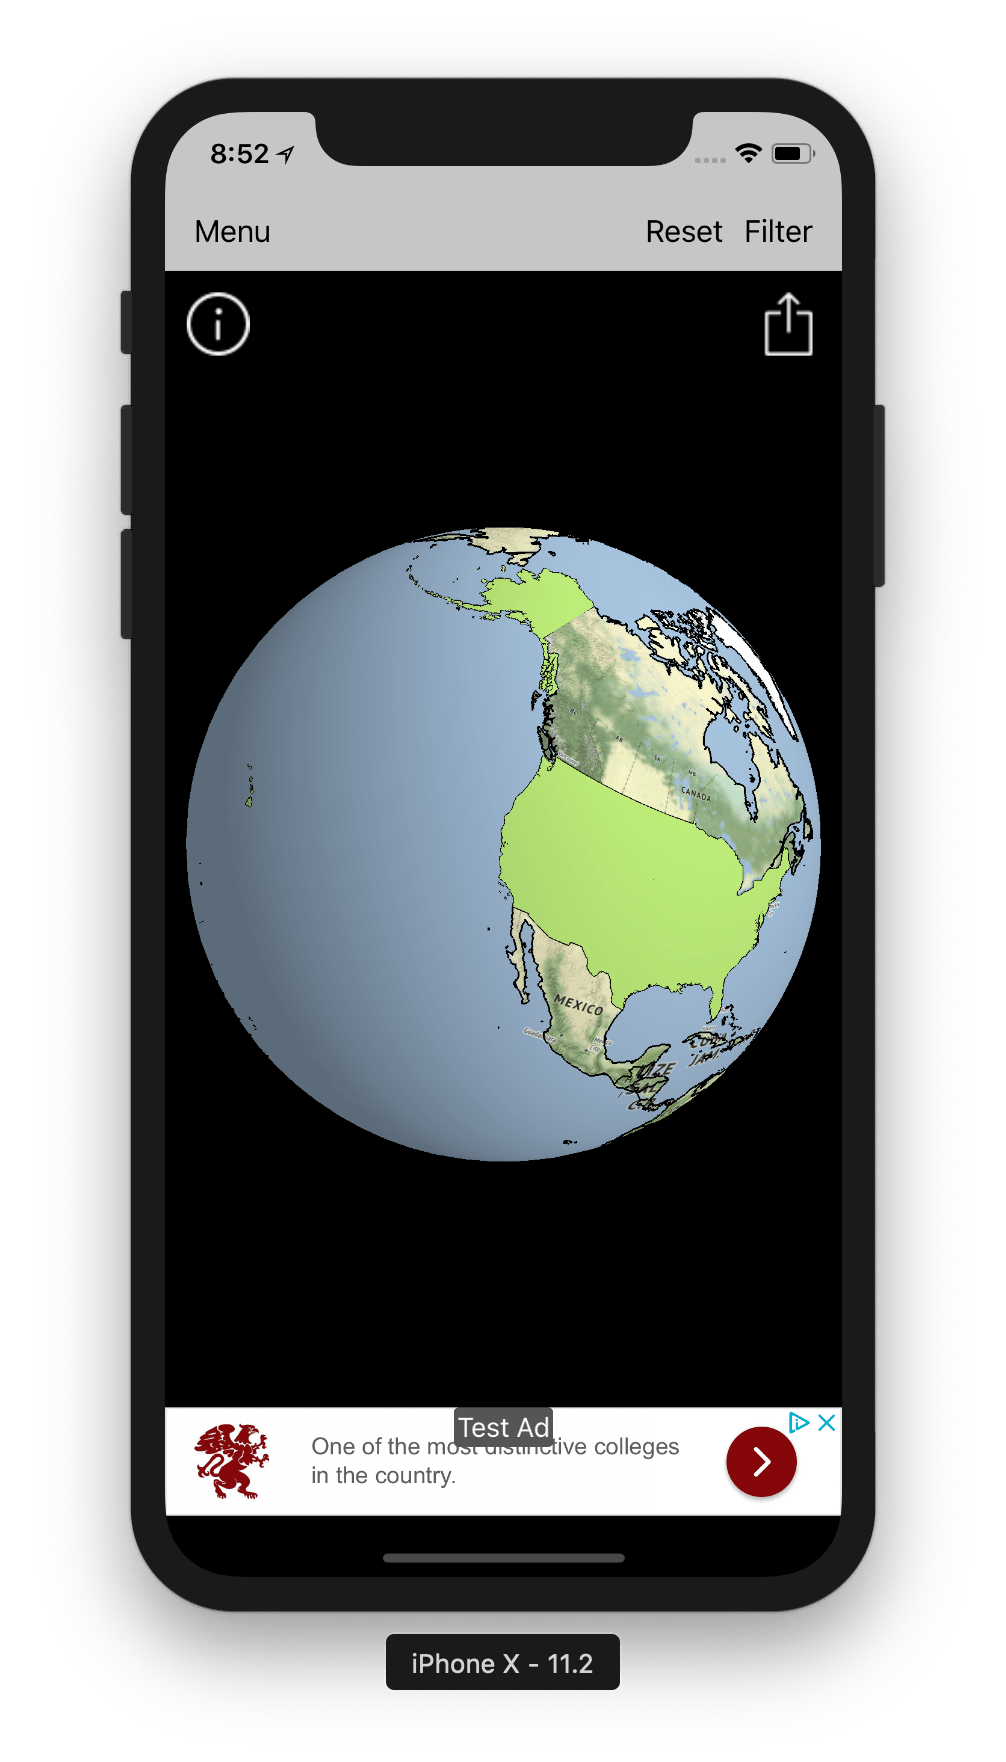
\includegraphics[width=0.25\linewidth]{figures/ch5/buttons.png}
            \caption{\label{fig:buttons} Home screen with two buttons on top corners}
        \end{figure}
     
    \item Left button in figure 5.1 corresponds to Info button which shows information about the current data that is being displayed. Figure 5.2 shows the view appears on tapping of information button. \\
    
      \begin{figure}[H]
            \centering
            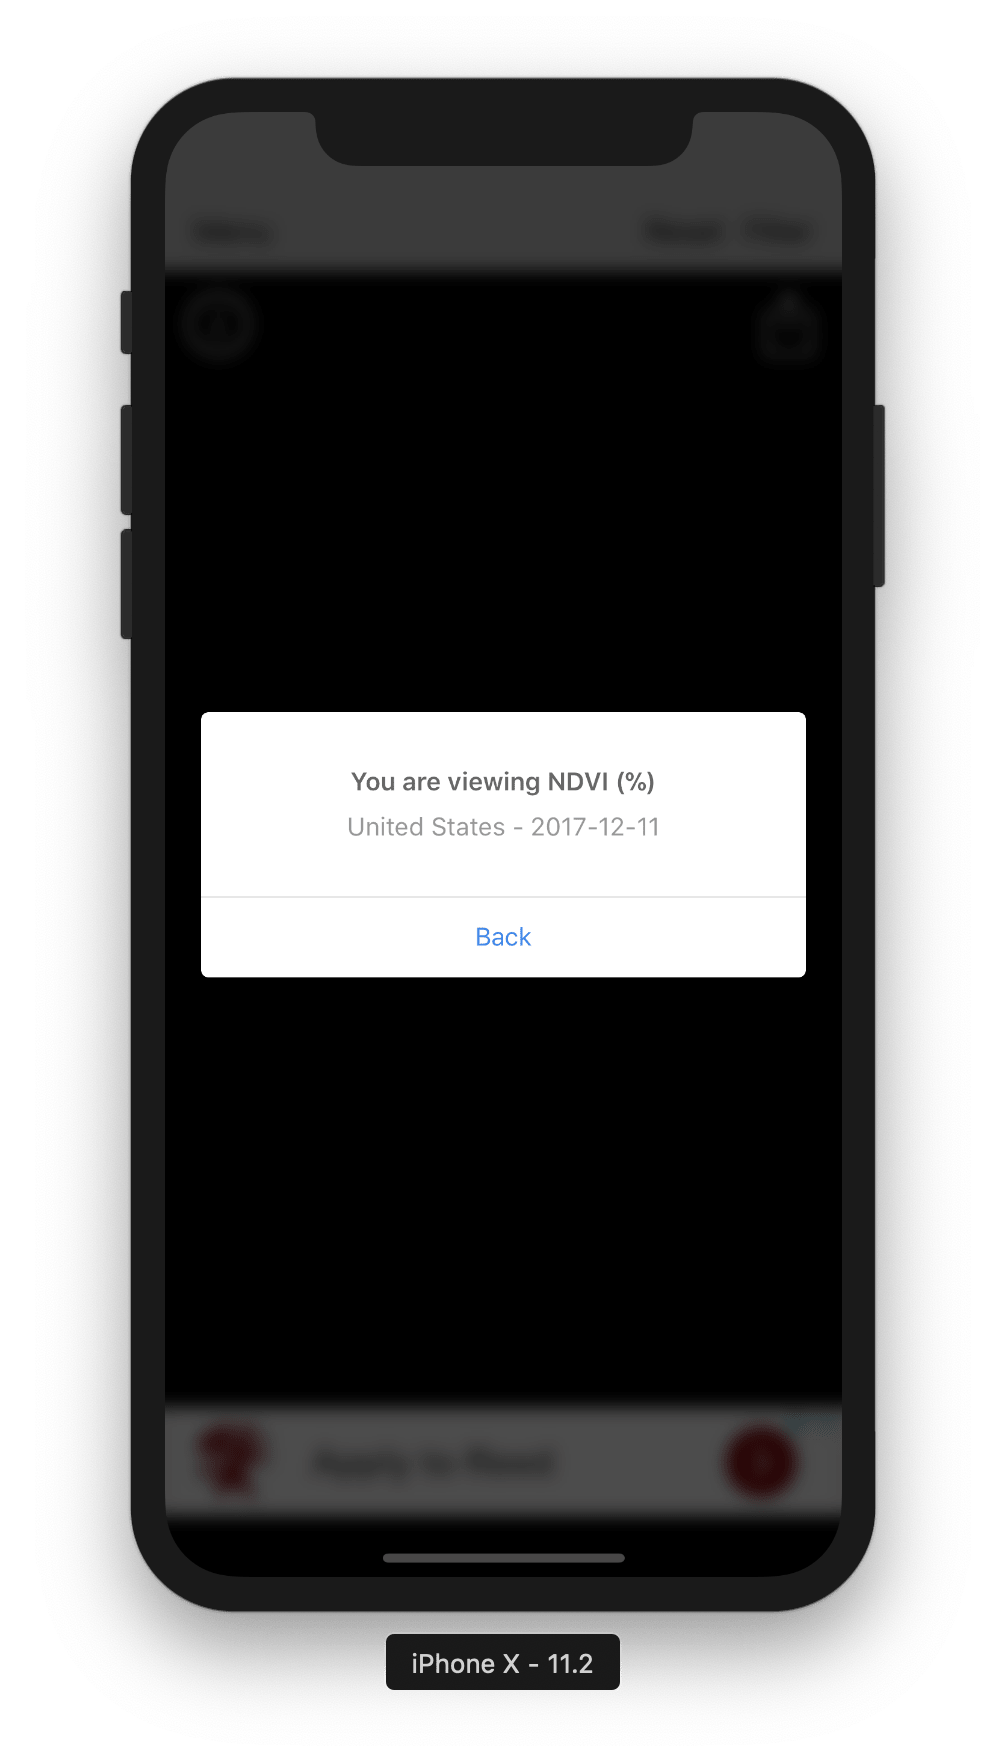
\includegraphics[width=0.25\linewidth]{figures/ch5/info_view.png}
            \caption{\label{fig:info_button} Information button action}
        \end{figure}
       
     \item Right button in figure 5.1 corresponds to export button which prompts you for exporting current data which is visible on globe / map. Figure 5.3 shows the export view on tapping of export button. \\
     
     \begin{figure}[H]
            \centering
            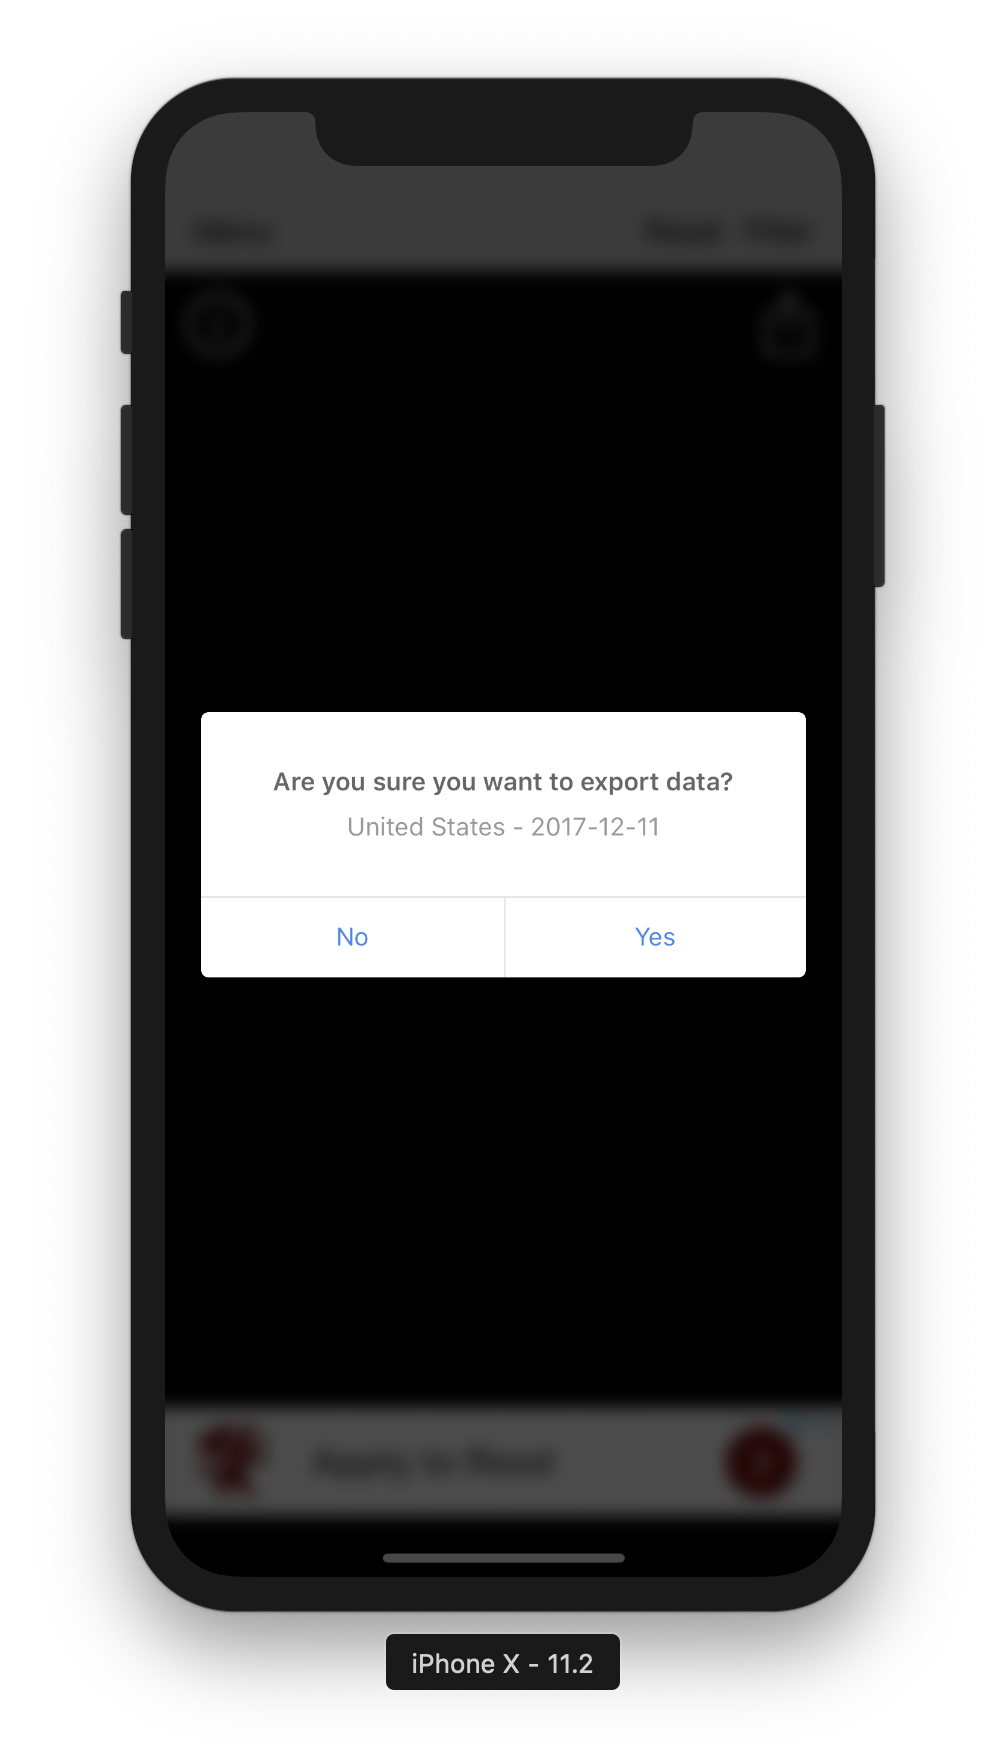
\includegraphics[width=0.25\linewidth]{figures/ch5/export_view.png}
            \caption{\label{fig:info_button} Export button action on home screen}
    \end{figure}
    
    On selecting yes in the figure 5.3, it then converts the raw \gls{json} data to a valid \gls{csv} format and attaches it as a file on the MFMailComposeViewController. \\
    
    
    According to Apple, It's a standard interface for managing, editing, and sending an email message in \gls{iOS} app. \cite{MFMailComposer} Figure 5.4 shows the MFMailComposerViewController view which helps user to email the \gls{csv} file. 
    
    \begin{figure}[H]
            \centering
            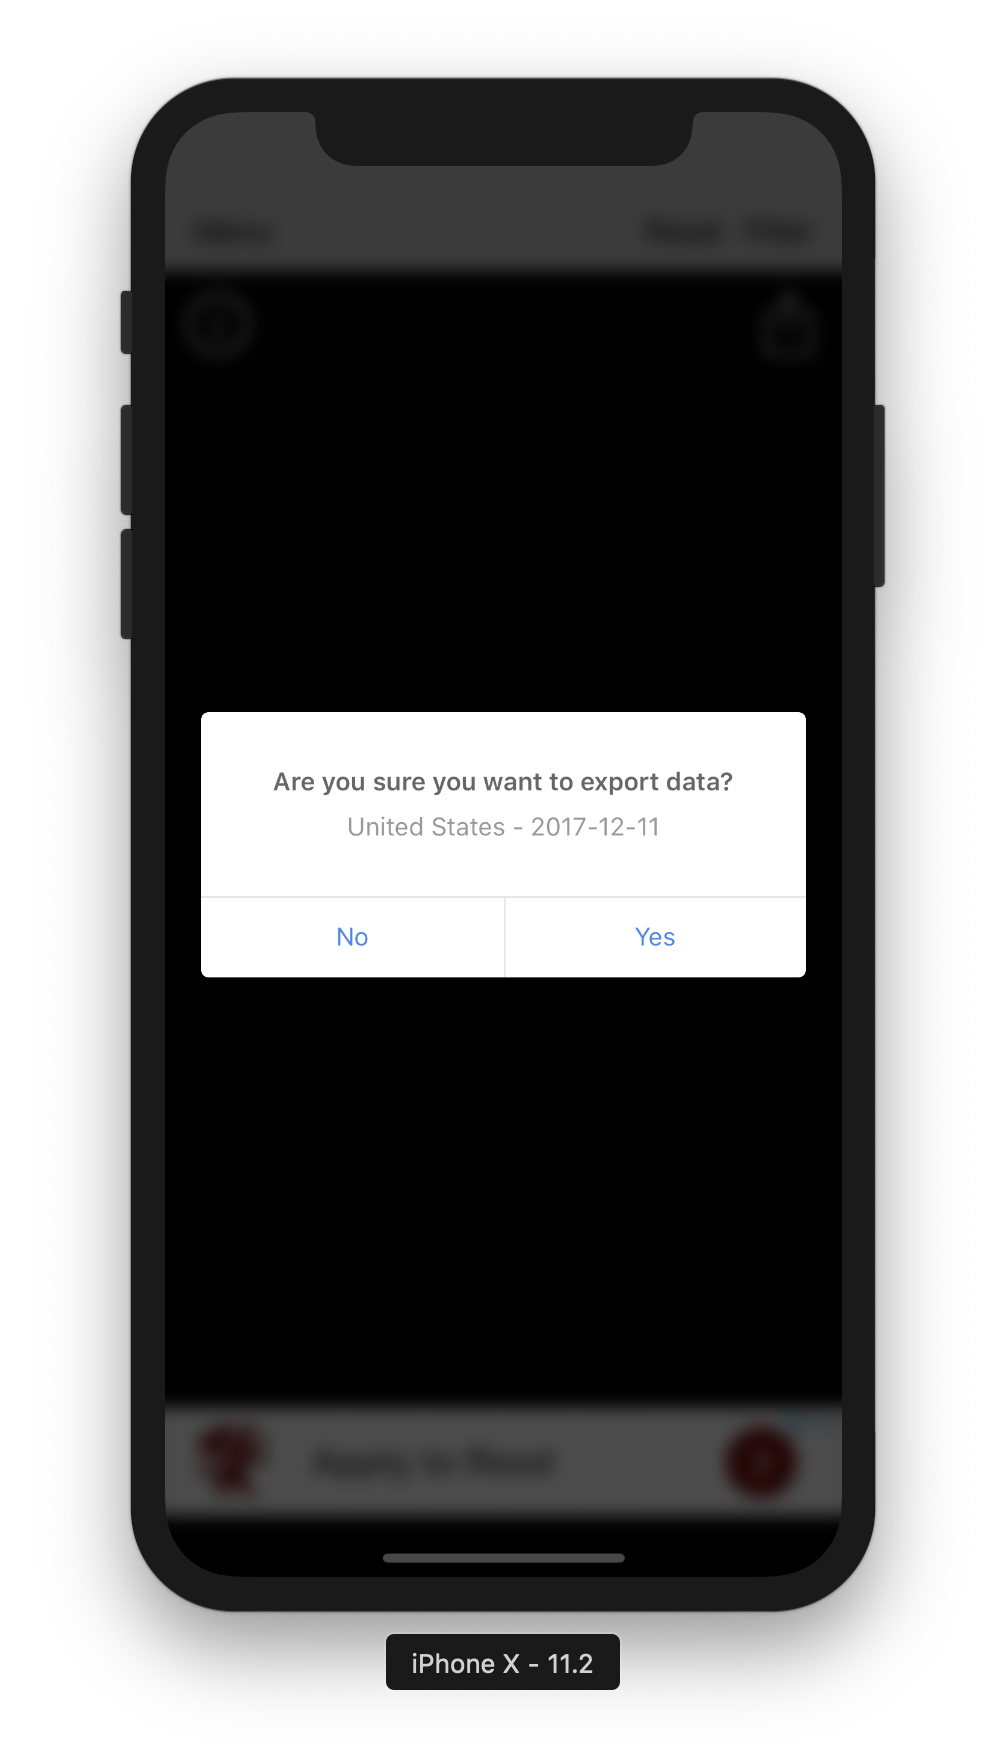
\includegraphics[width=0.25\linewidth]{figures/ch5/export_view.png}
            \caption{\label{fig:info_button} Email controller after selecting yes on export action screen}
    \end{figure}
    
\end{itemize}

\newpage

\section{Computing mean, Standard Deviation, histograms}

\begin{itemize}
    \item \textbf{Mean} \\
    According to a paper published in 1997, The mean of a data set is simply the arithmetic average of the values in the set, obtained by summing the values and dividing by the number of values. Recall that when we summarize a data set in a frequency distribution, we are approximating the data set by "rounding" each value in a given class to the class mark. With this in mind, it is natural to define the mean of a frequency distribution by figure 5.5. \cite{Mean_SD}
    
     \begin{figure}[H]
            \centering
            
\includegraphics[width=0.25\linewidth]{figures/ch5/mean_formula.png}
            \caption{\label{fig:info_button} Mean formula}
    \end{figure}
    
    \item \textbf{Standard Deviation} \\
   It is defined as the amount computed to show the degree of deviation for a gathering all in all.
    
     \begin{figure}[H]
            \centering
            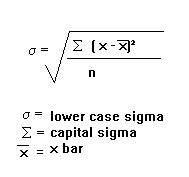
\includegraphics[width=0.25\linewidth]{figures/ch5/standard_deviation.png}
            \caption{\label{fig:info_button} Standard deviation formula}
    \end{figure}
    
\end{itemize}

\centerline{\textbf{Why use mean and standard deviation for analysis?}}

The main purpose of using mean and standard deviation as a parameter for analysis is that the Normal Curve discloses to us that numerical data will be disseminated in an pattern around a normal line whereas Standard deviation is viewed as the most valuable list of variability. It is a solitary number that discloses to us the inconstancy, or spread, of an appropriation (gathering of scores).

We have investigated \gls{ndvi} and Anomaly a portion of the nations just to demonstrate that with the sent out information through the app, client can do these things:

\newpage

\begin{itemize}
    \item \textbf{Mean NDVI \& Anomaly distribution over the years}
    
    \begin{figure}[!htb]
        \begin{minipage}{0.5\textwidth}
            \centering
            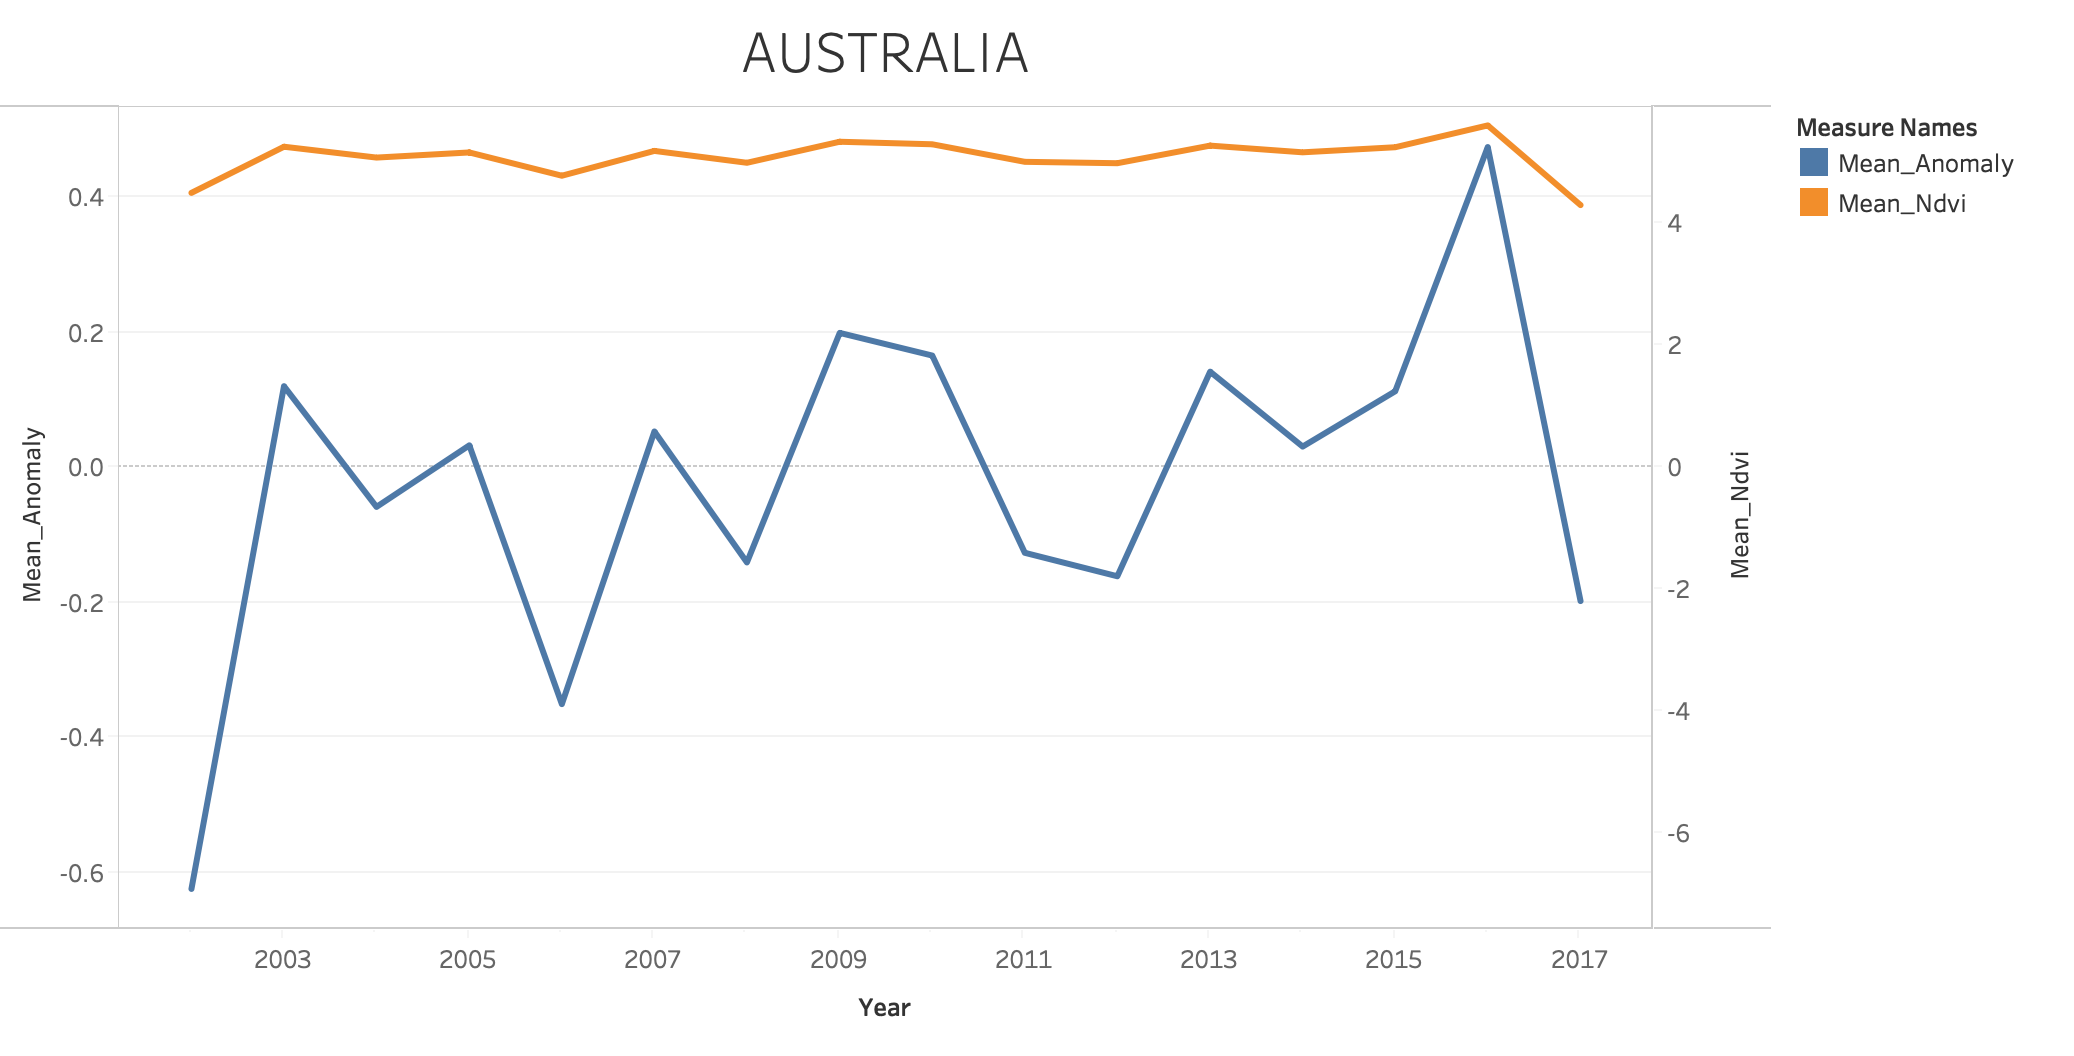
\includegraphics[width=1.0\linewidth]{figures/ch5/Mean/AUSTRALIA_mean.png}
            \caption{Mean graph - Australia}\label{Fig:AUSTRALIA_mean}
        \end{minipage}\hfill
        \begin{minipage}{0.5\textwidth}
            \centering
            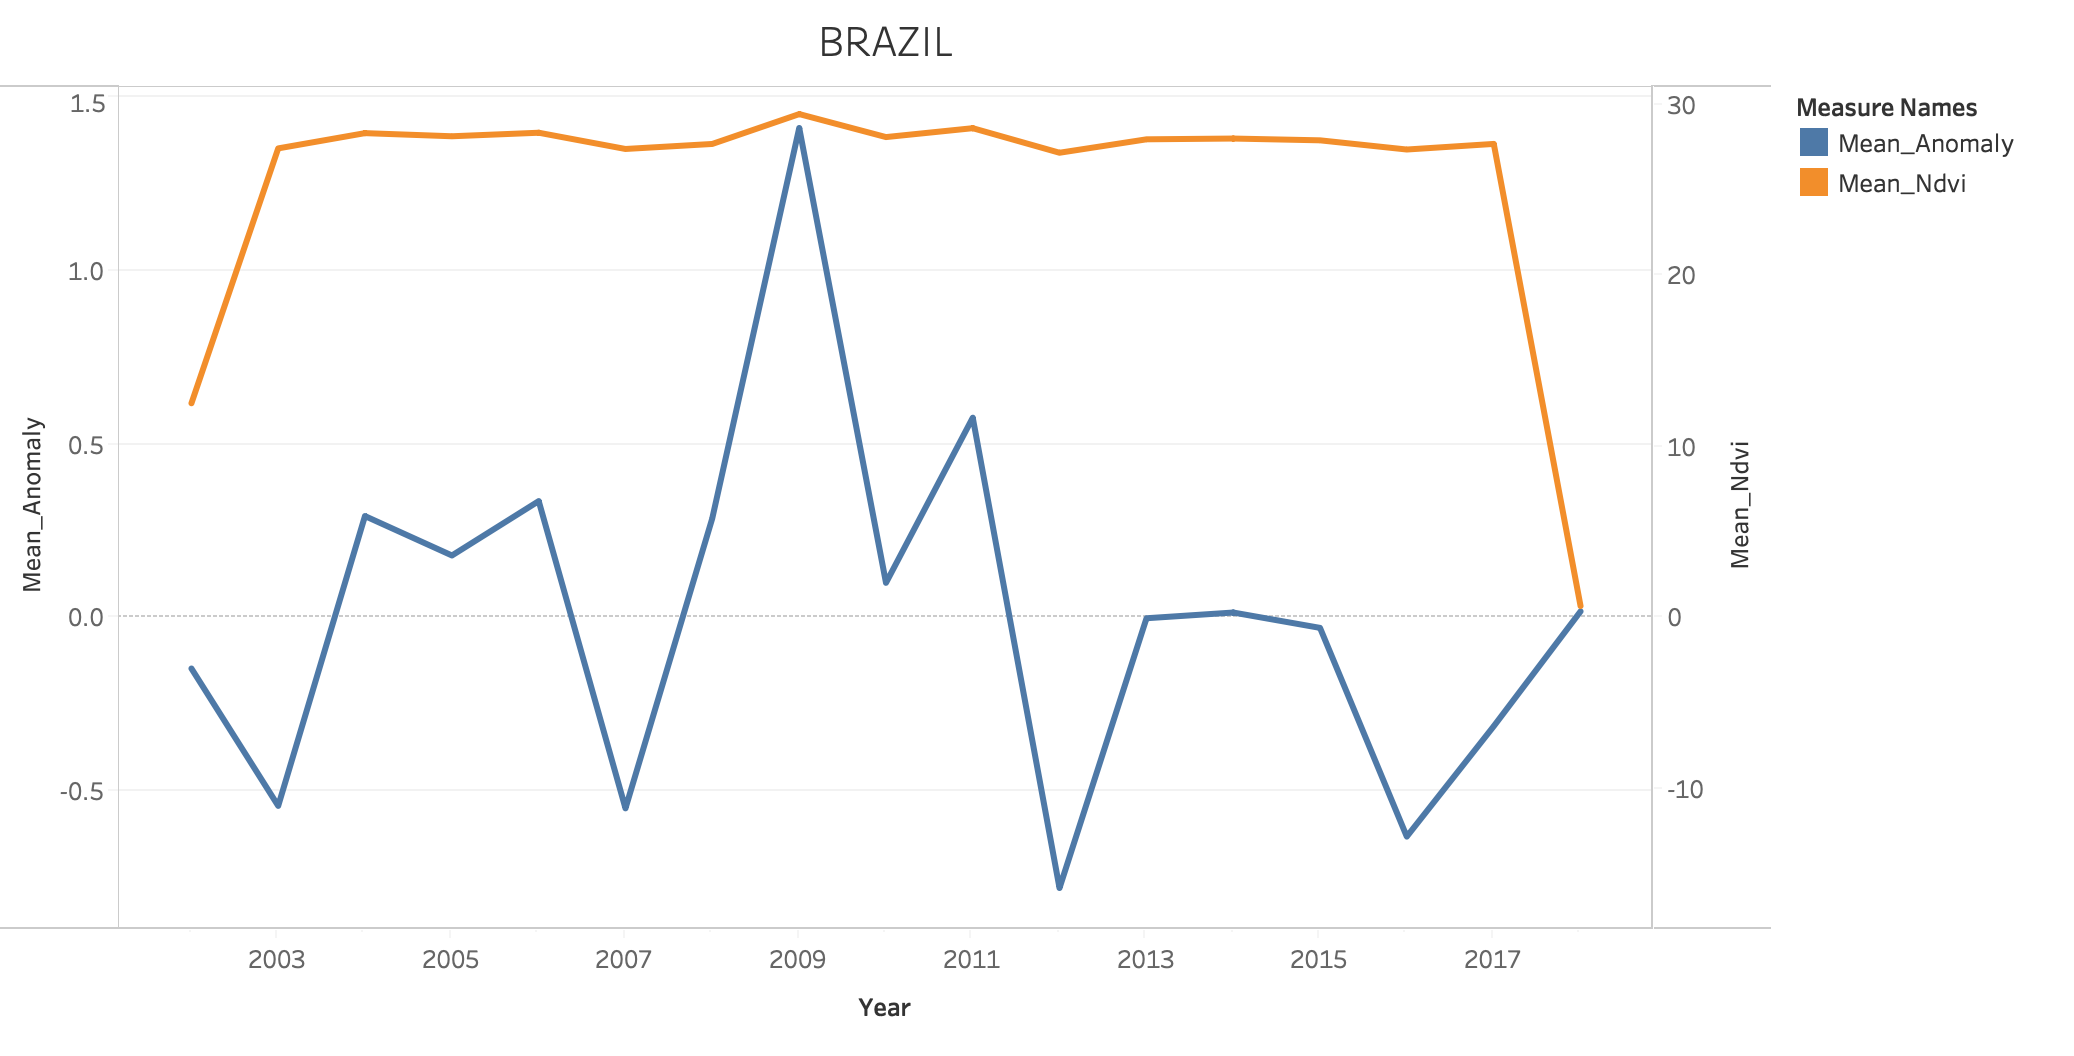
\includegraphics[width=1.0\linewidth]{figures/ch5/Mean/BRAZIL_mean.png}
            \caption{Mean graph - Brazil}\label{Fig:BRAZIL_mean}
        \end{minipage}
    \end{figure}
    
     \begin{figure}[!htb]
        \begin{minipage}{0.5\textwidth}
            \centering
            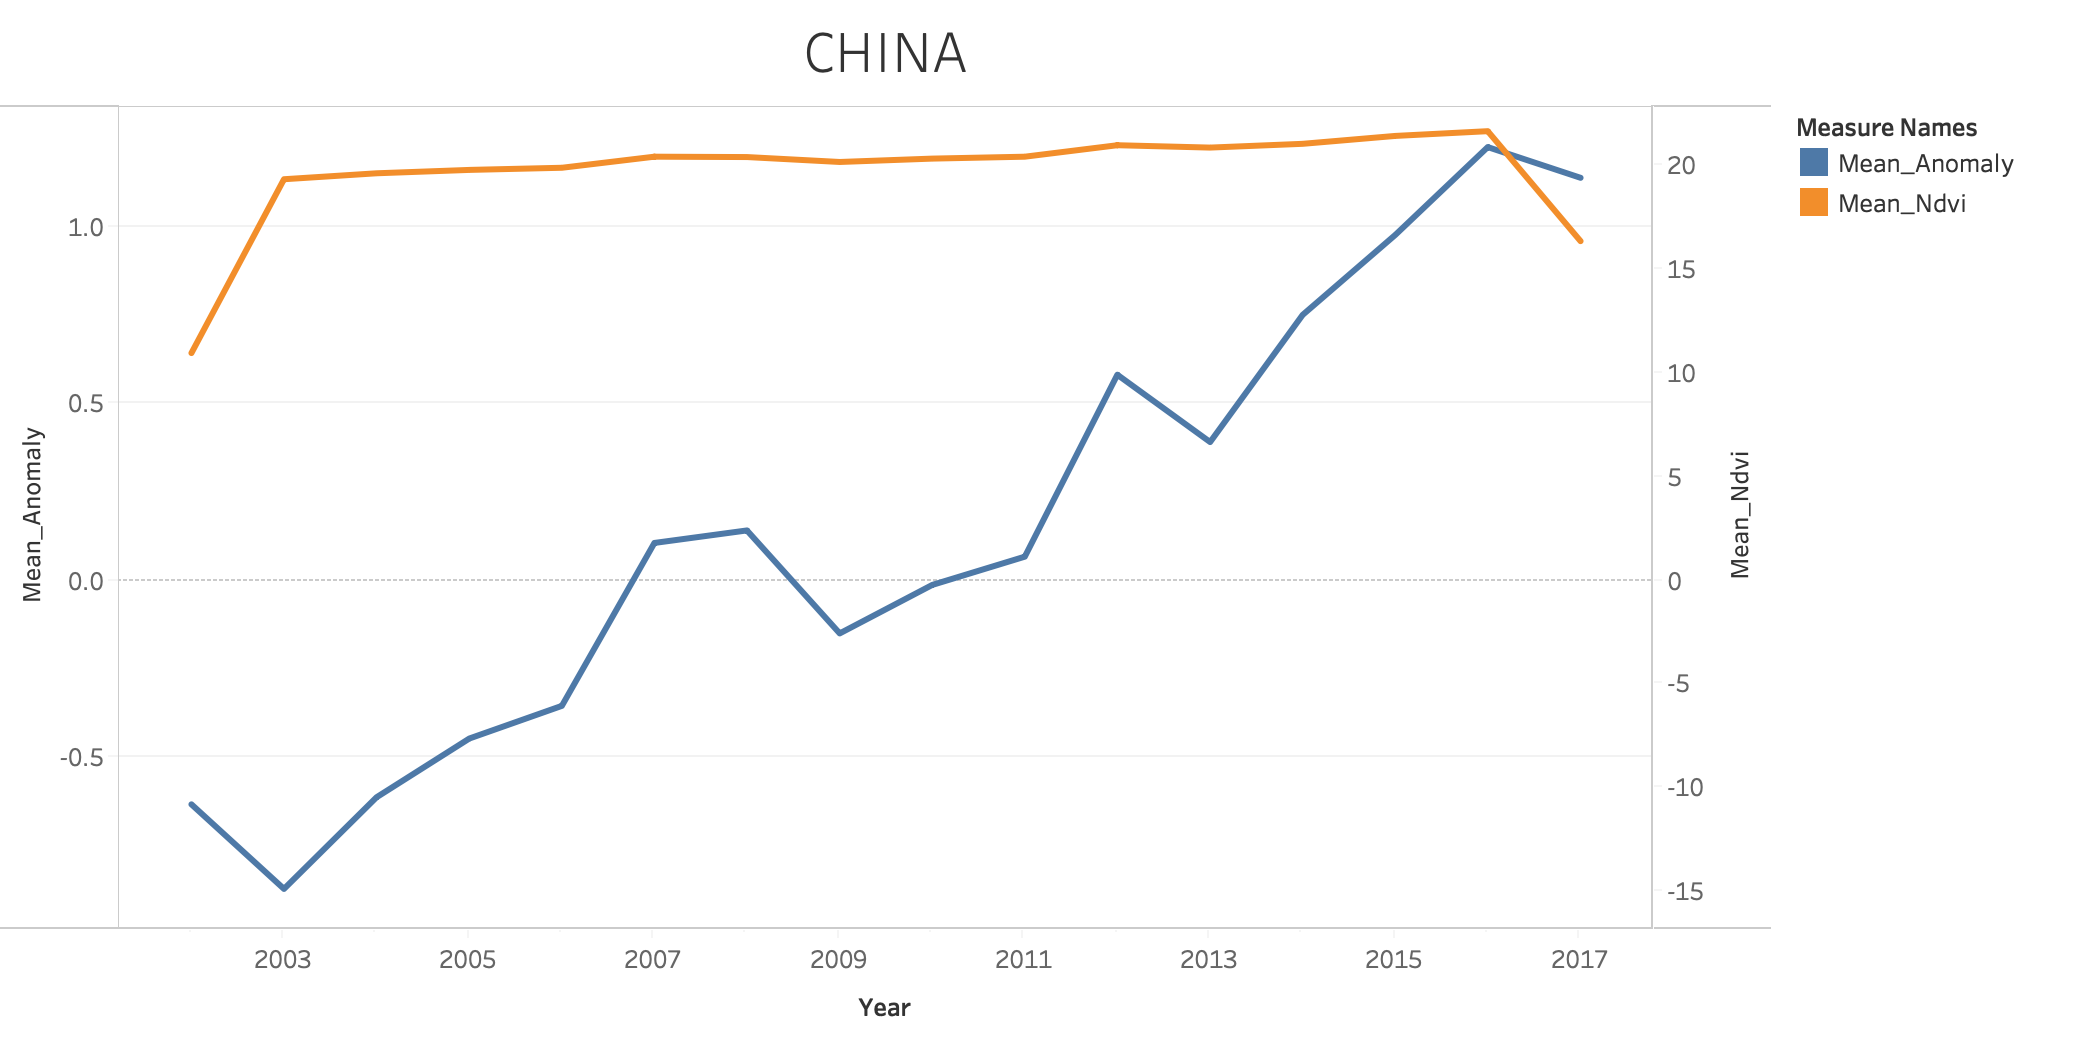
\includegraphics[width=1.0\linewidth]{figures/ch5/Mean/CHINA_mean.png}
            \caption{Mean - China}\label{Fig:CHINA_mean}
        \end{minipage}\hfill
        \begin{minipage}{0.5\textwidth}
            \centering
            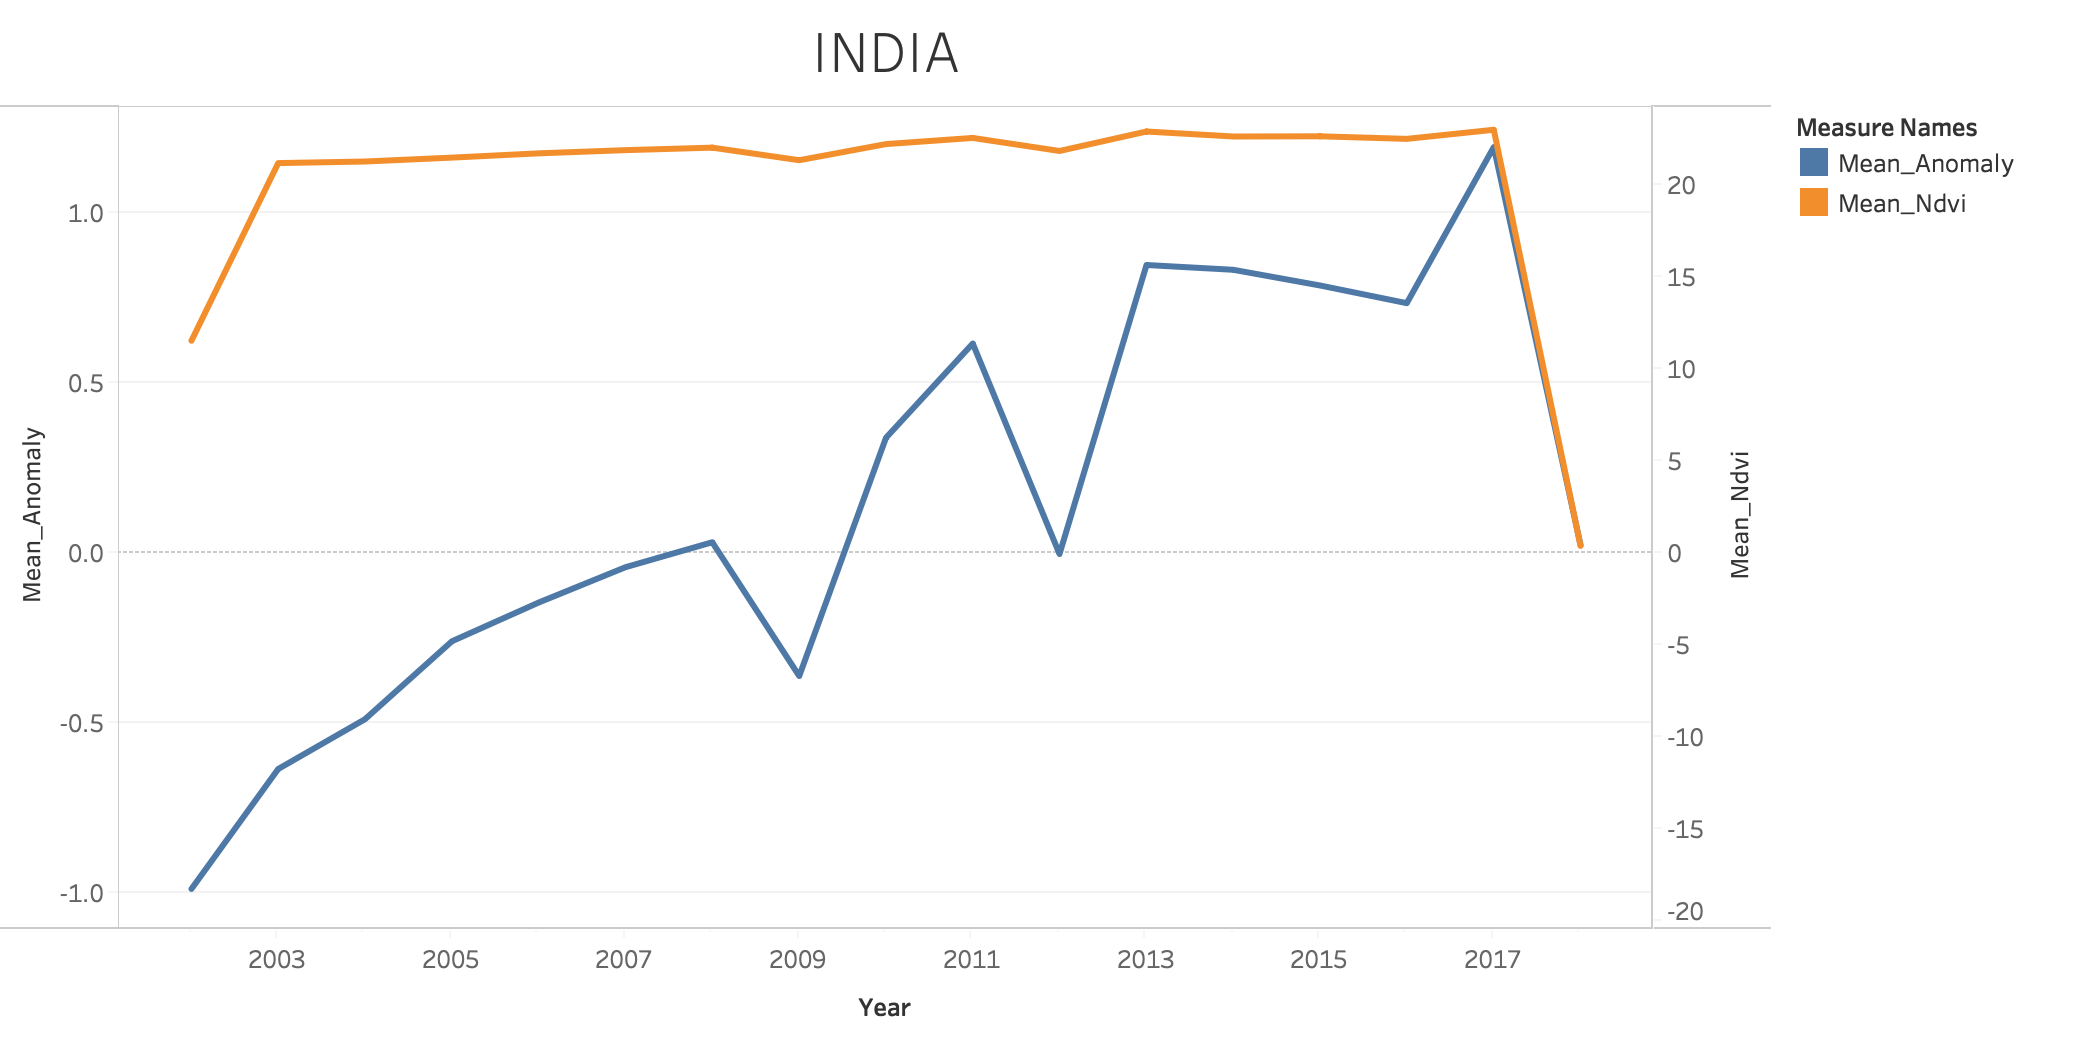
\includegraphics[width=1.0\linewidth]{figures/ch5/Mean/INDIA_mean.png}
            \caption{Mean graph - India}\label{Fig:INDIA_mean}
        \end{minipage}
    \end{figure}
    
     \begin{figure}[H]
            \centering
            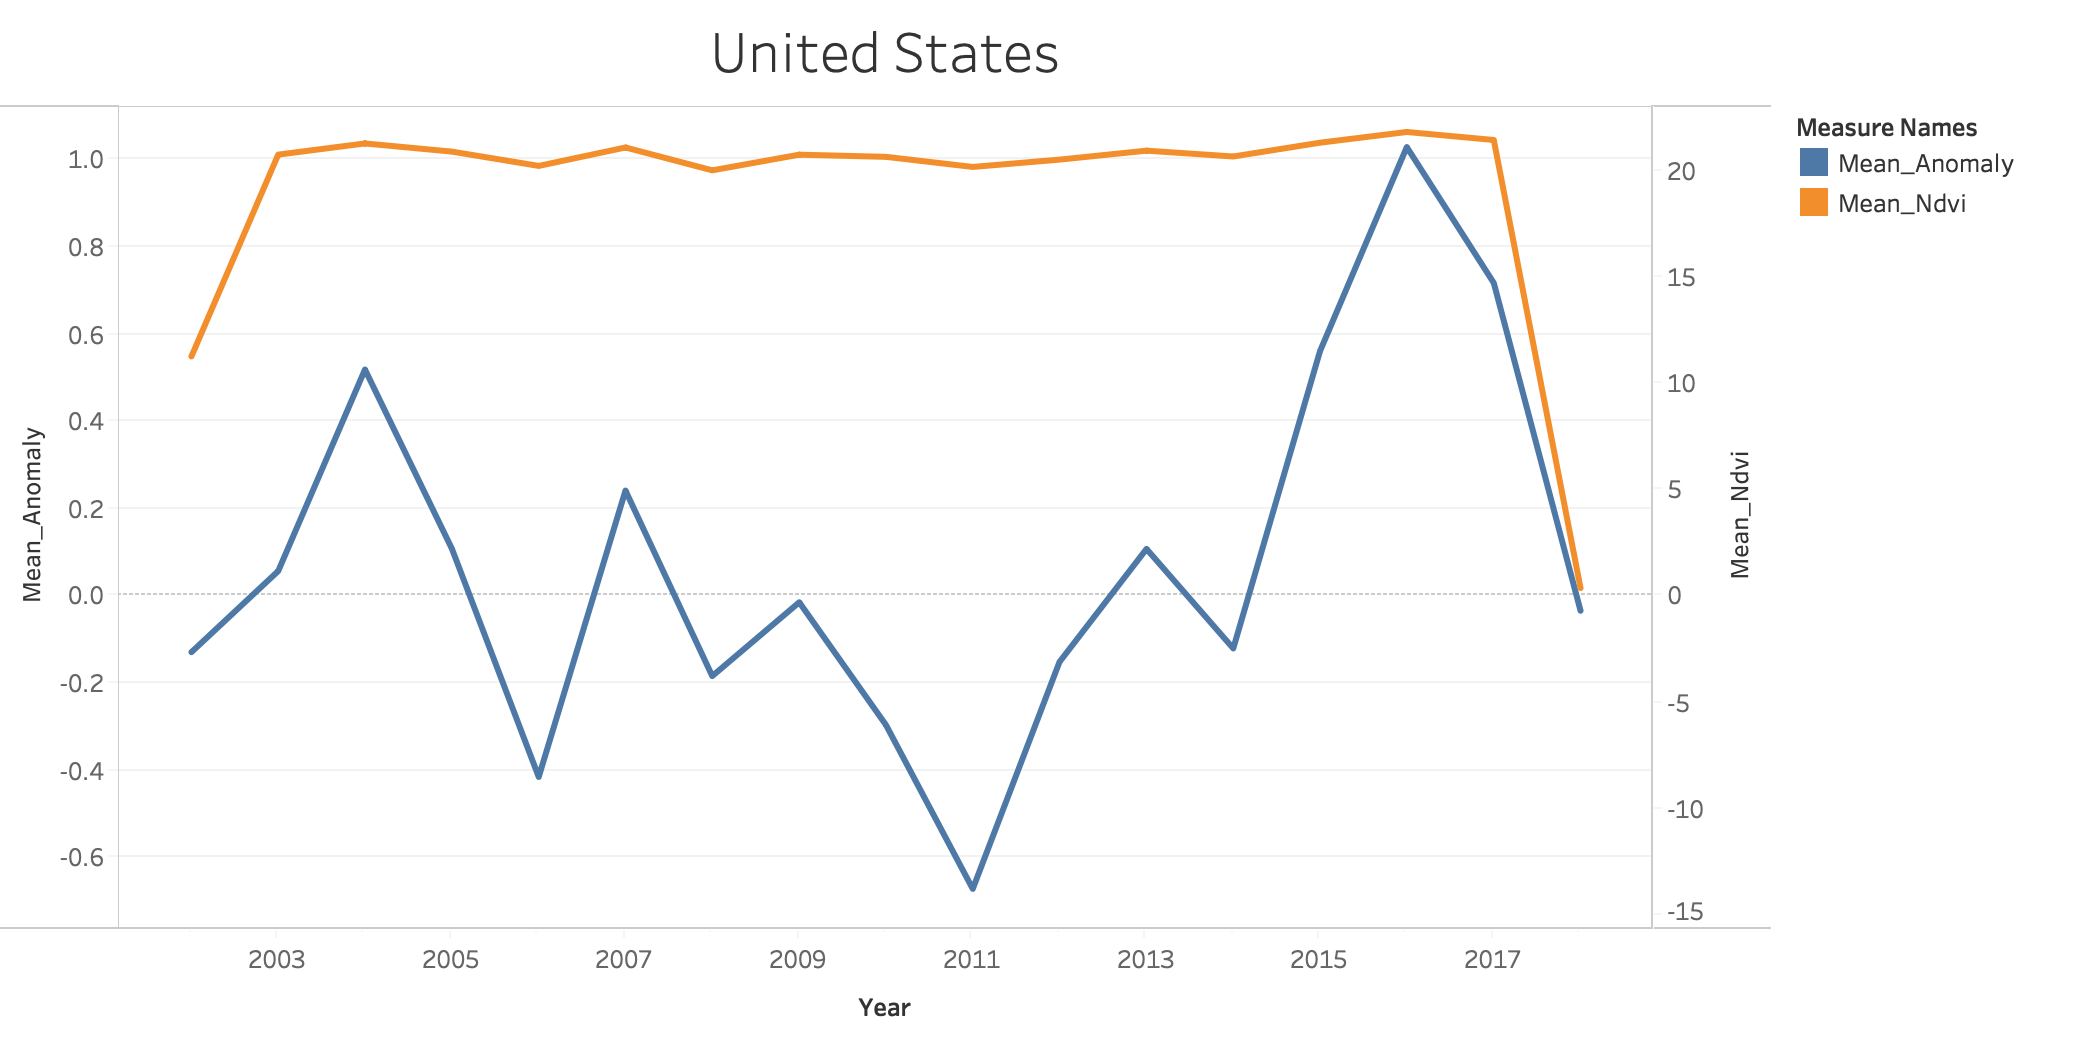
\includegraphics[width=0.5\linewidth]{figures/ch5/Mean/US_mean.png}
            \caption{\label{fig:US_mean}Mean graph - United States}
    \end{figure}

    \clearpage
    \newpage

    \item \textbf{Standard Deviation NDVI \& Anomaly distribution over the years}

    \begin{figure}[!htb]
        \begin{minipage}{0.5\textwidth}
            \centering
            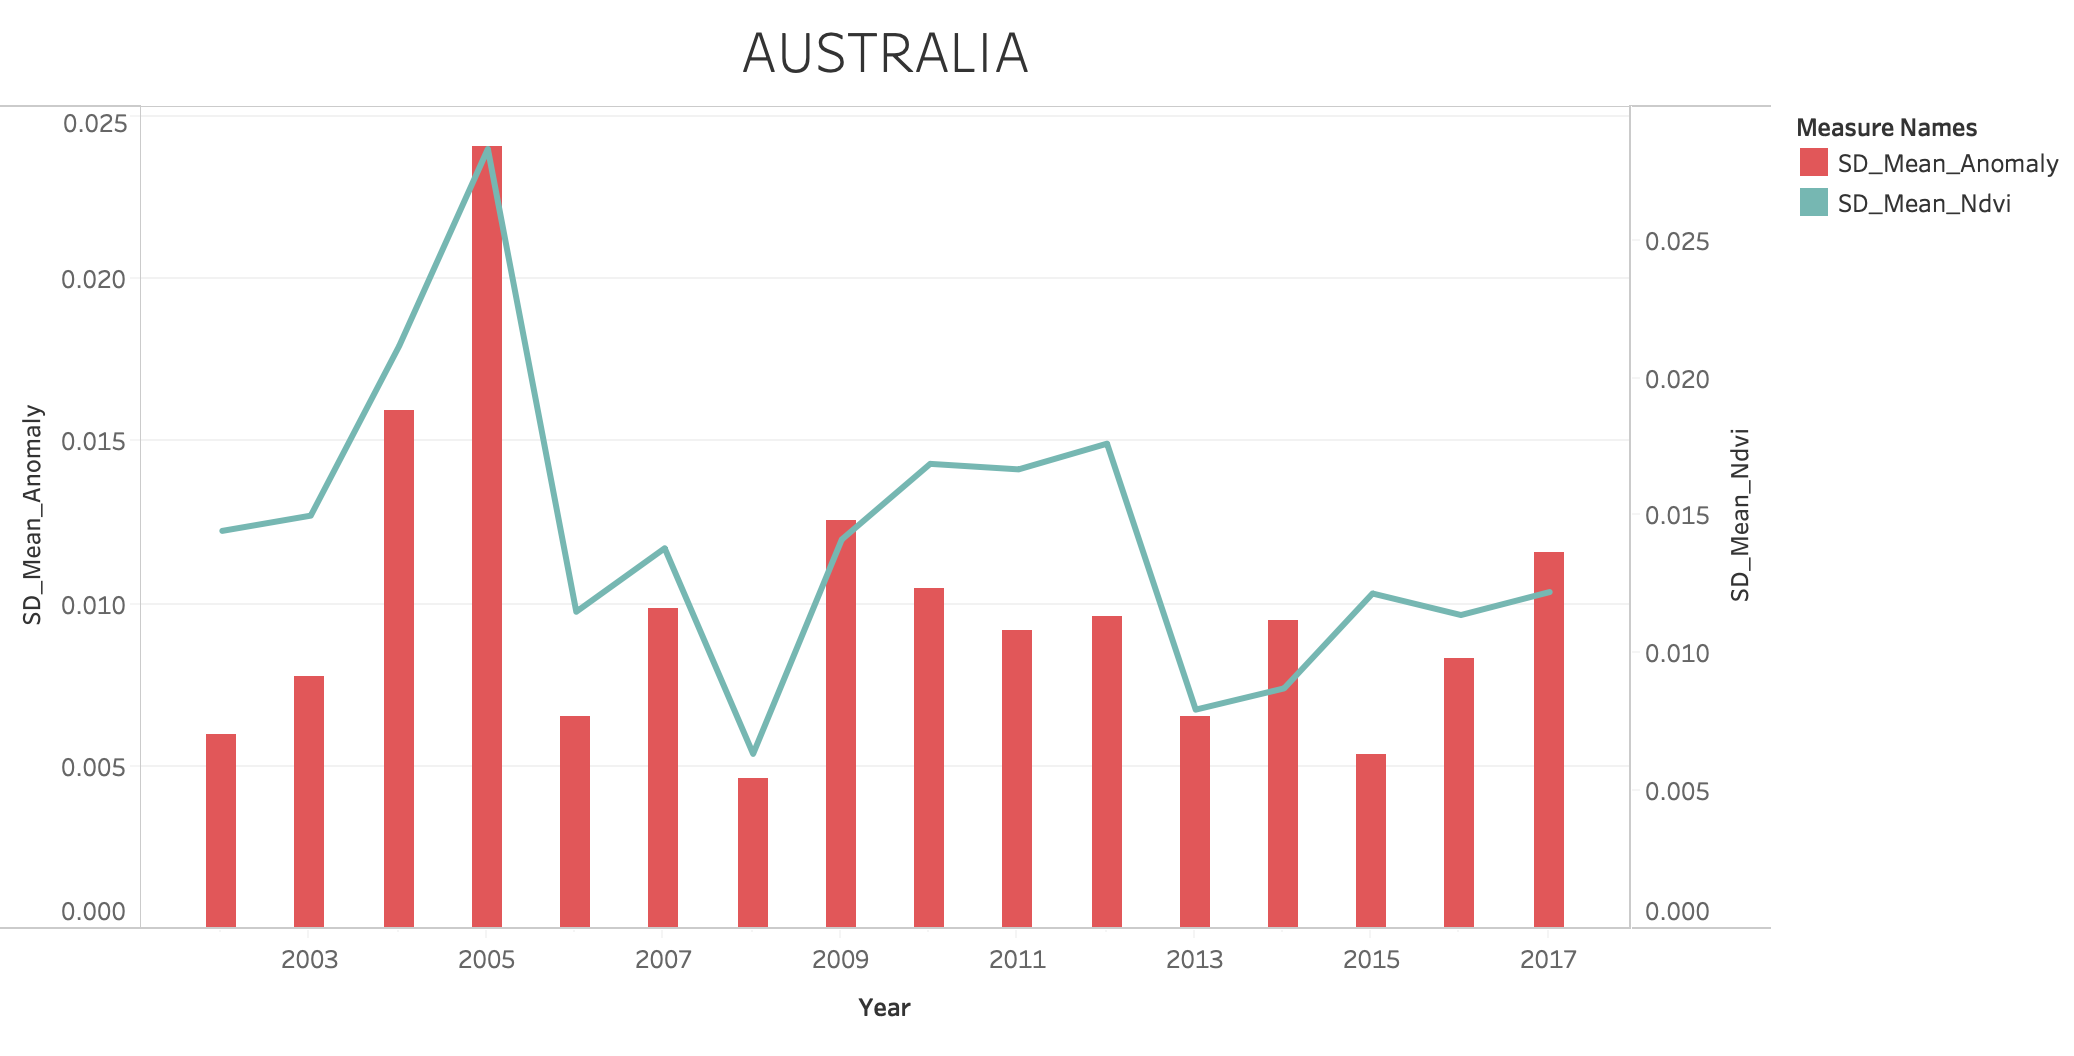
\includegraphics[width=1.0\linewidth]{figures/ch5/StandardDeviation/AUSTRALIA_SD.png}
            \caption{Standard deviation graph - Australia}\label{Fig:AUSTRALIA_SD}
        \end{minipage}\hfill
        \begin{minipage}{0.5\textwidth}
            \centering
            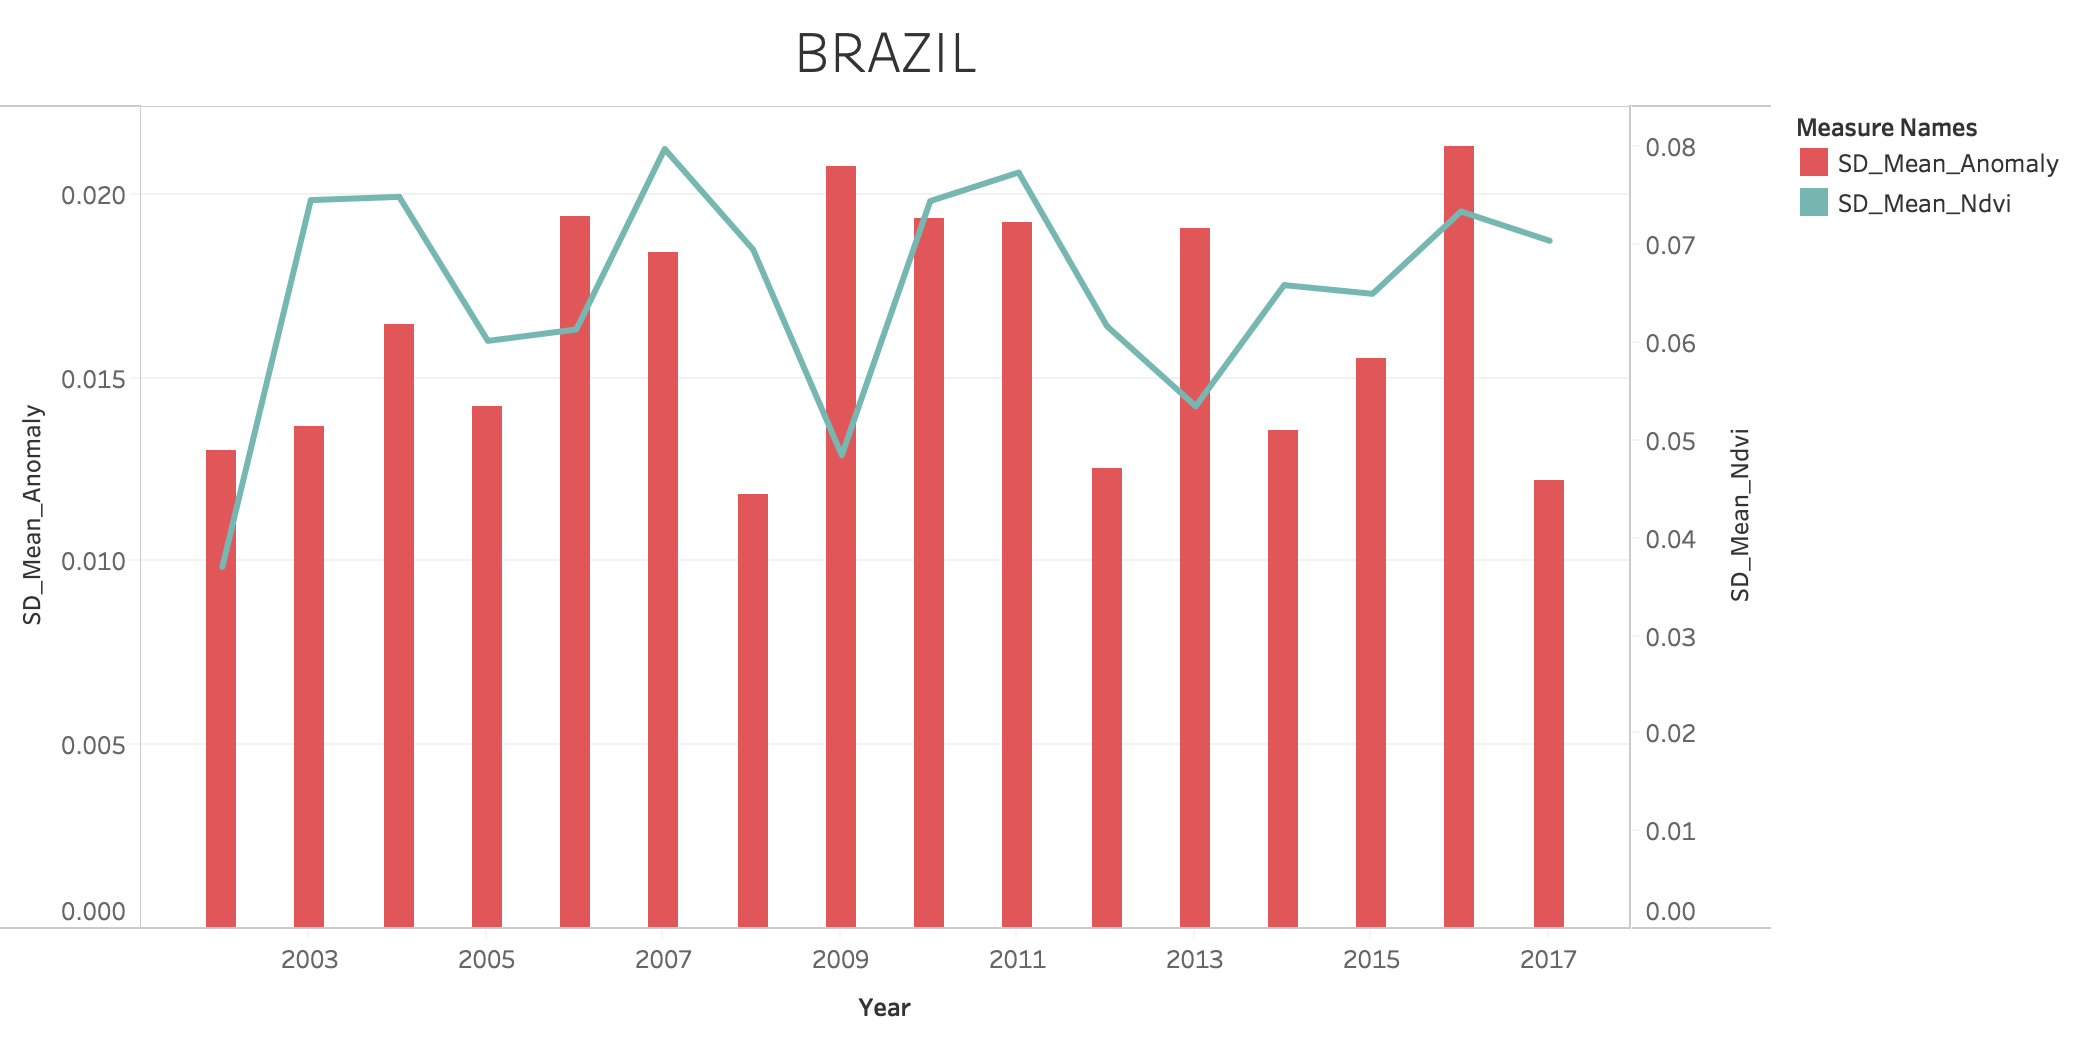
\includegraphics[width=1.0\linewidth]{figures/ch5/StandardDeviation/BRAZIL_SD.png}
            \caption{Standard deviation graph - Brazil}\label{Fig:BRAZIL_SD}
        \end{minipage}
    \end{figure}
    
     \begin{figure}[!htb]
        \begin{minipage}{0.5\textwidth}
            \centering
            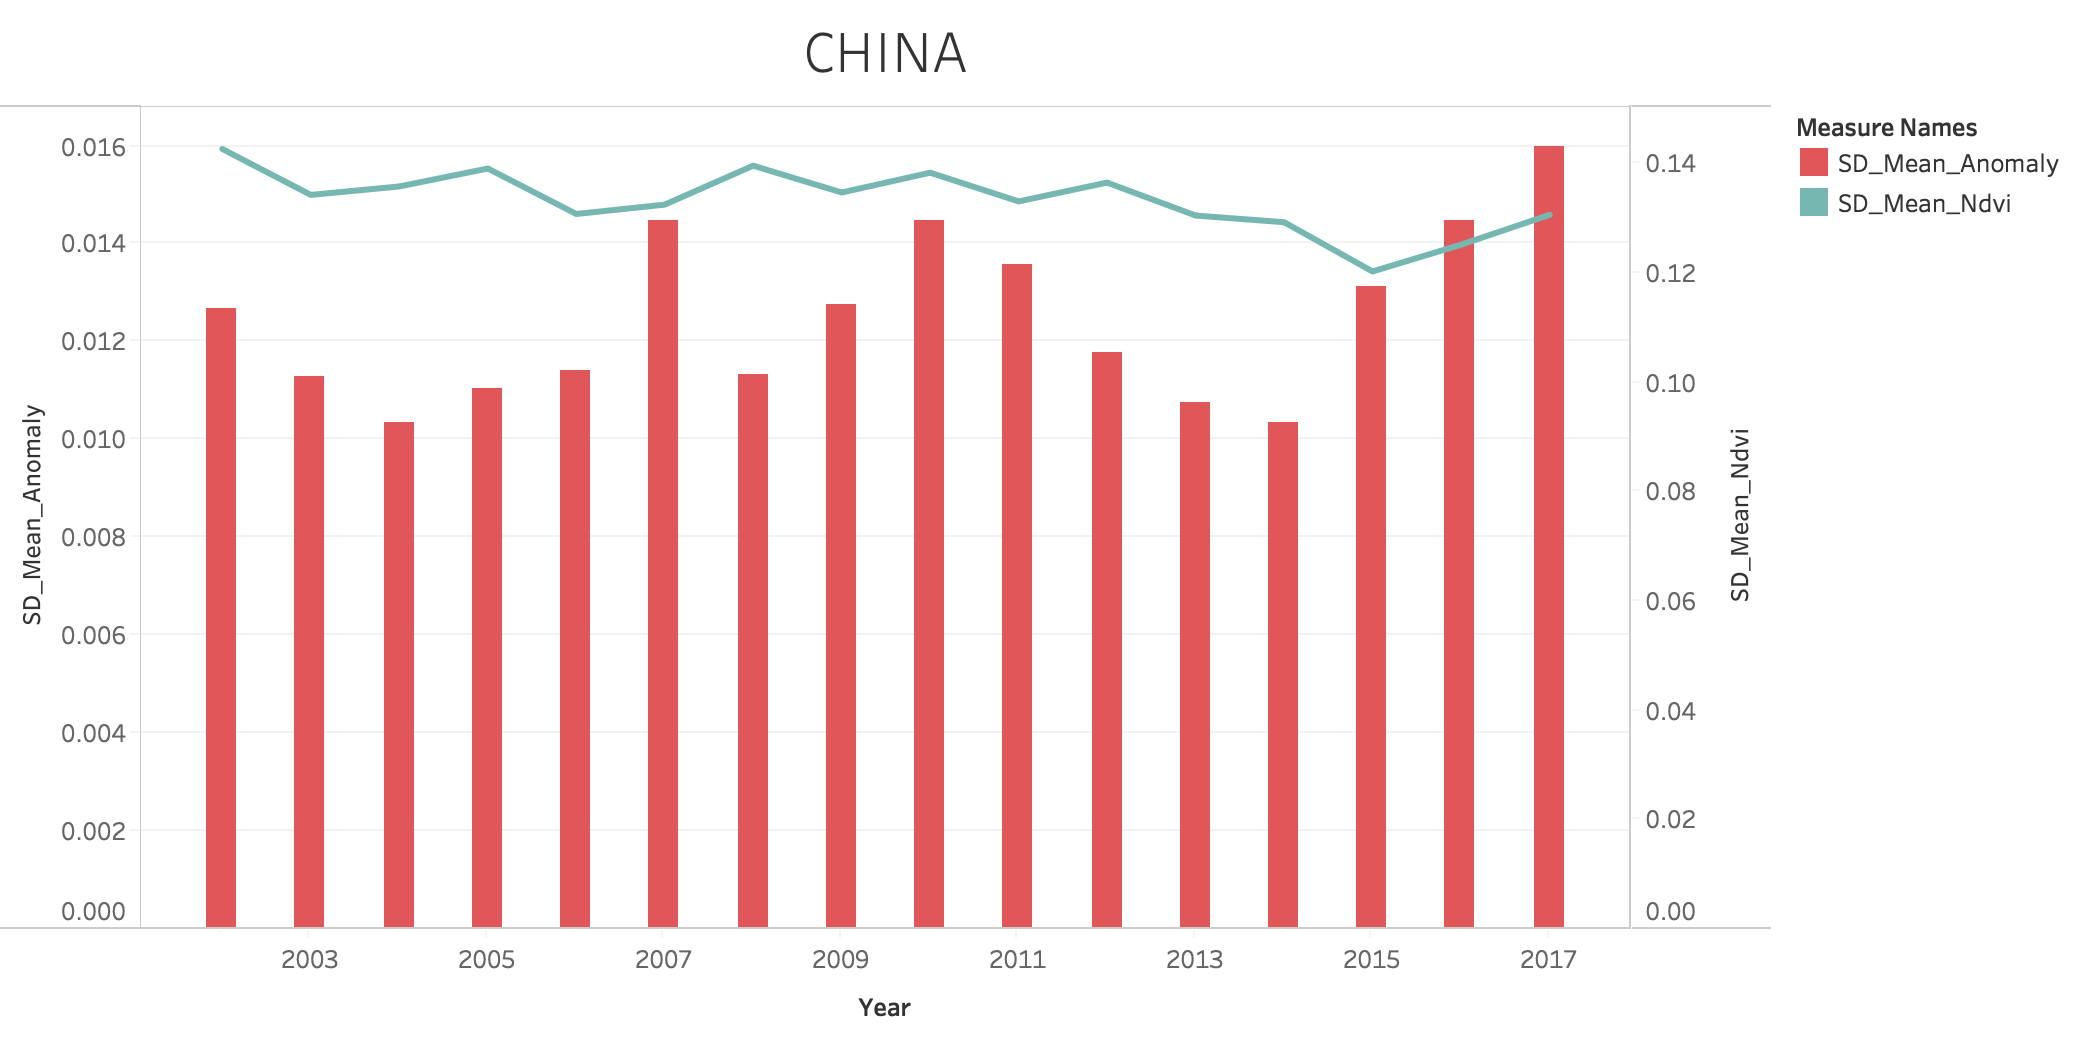
\includegraphics[width=1.0\linewidth]{figures/ch5/StandardDeviation/CHINA_SD.png}
            \caption{Standard deviation graph - China}\label{Fig:CHINA_SD}
        \end{minipage}\hfill
        \begin{minipage}{0.5\textwidth}
            \centering
            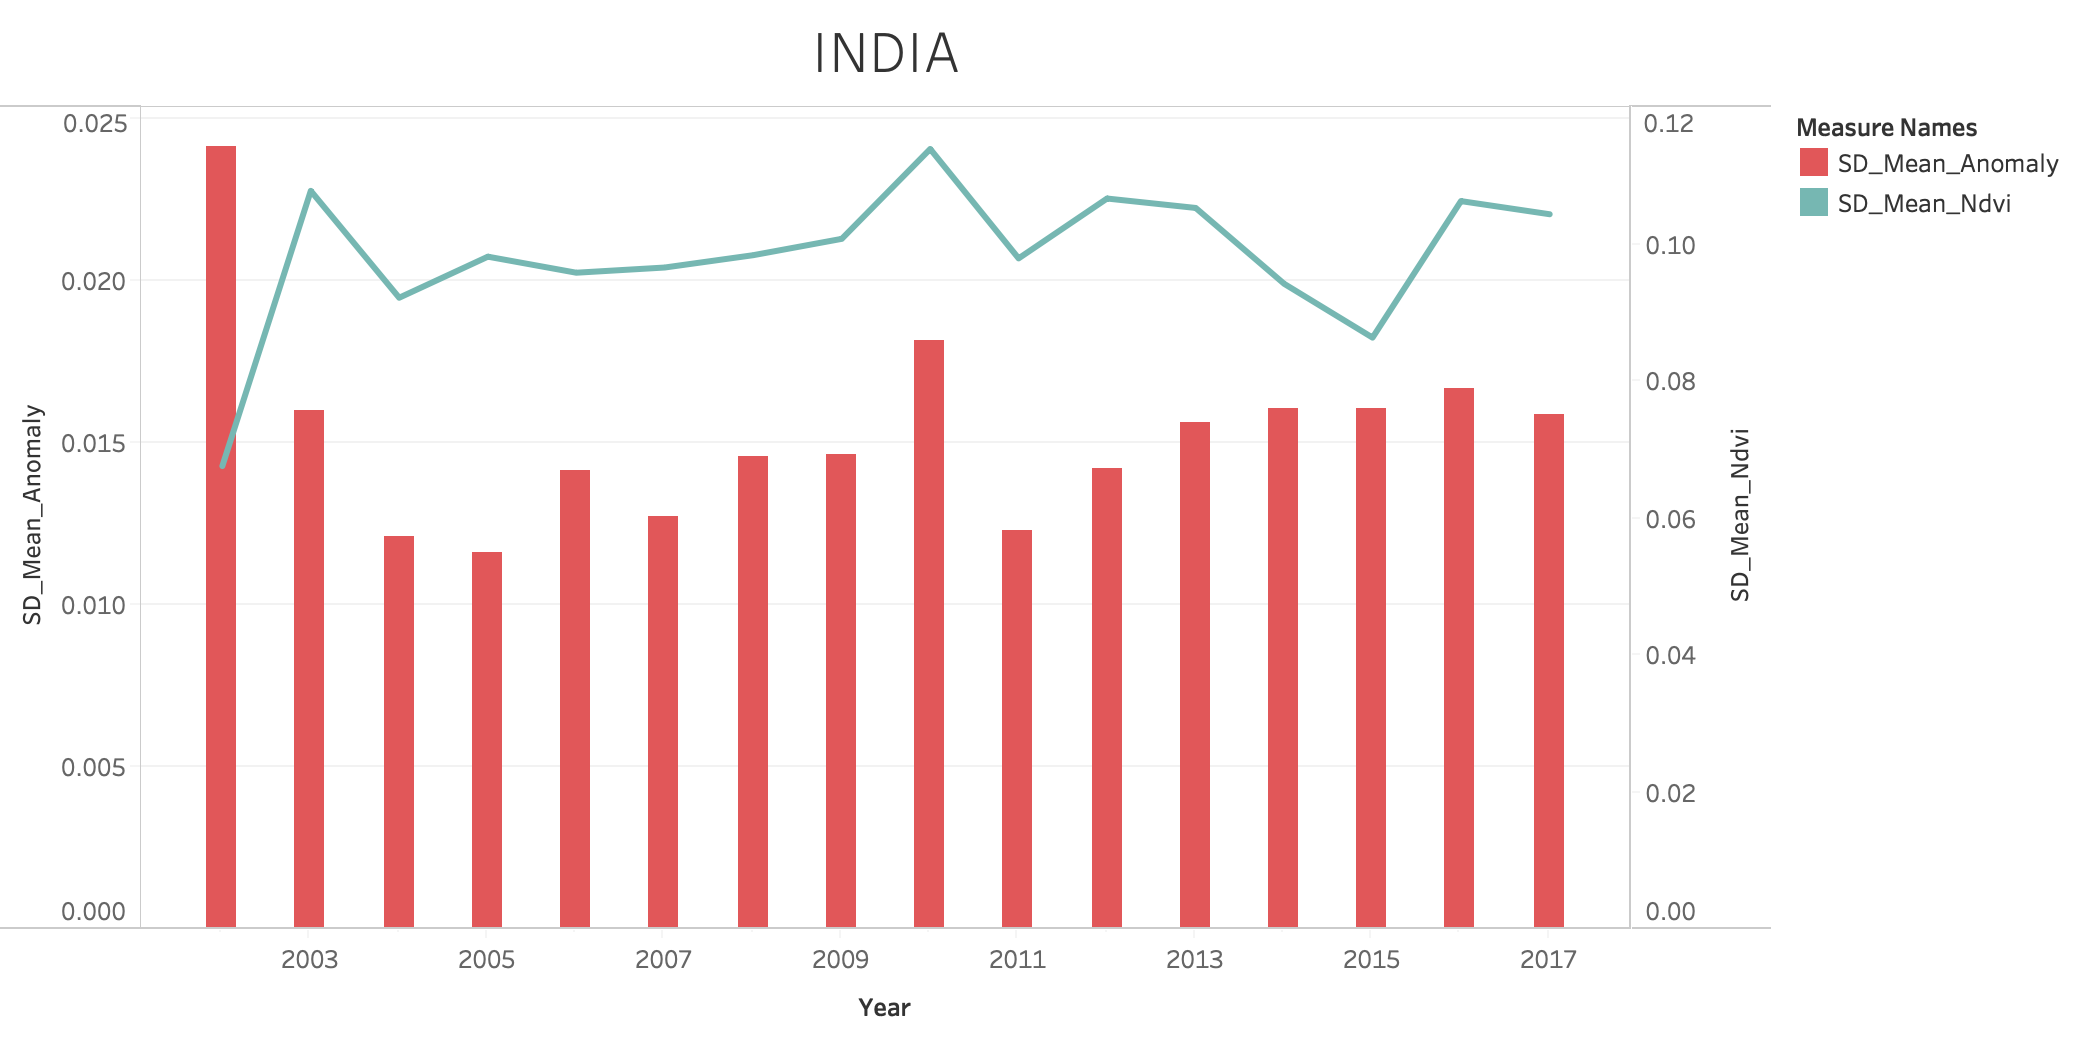
\includegraphics[width=1.0\linewidth]{figures/ch5/StandardDeviation/INDIA_SD.png}
            \caption{Standard deviation graph - India}\label{Fig:INDIA_SD}
        \end{minipage}
    \end{figure}
    
     \begin{figure}[H]
            \centering
            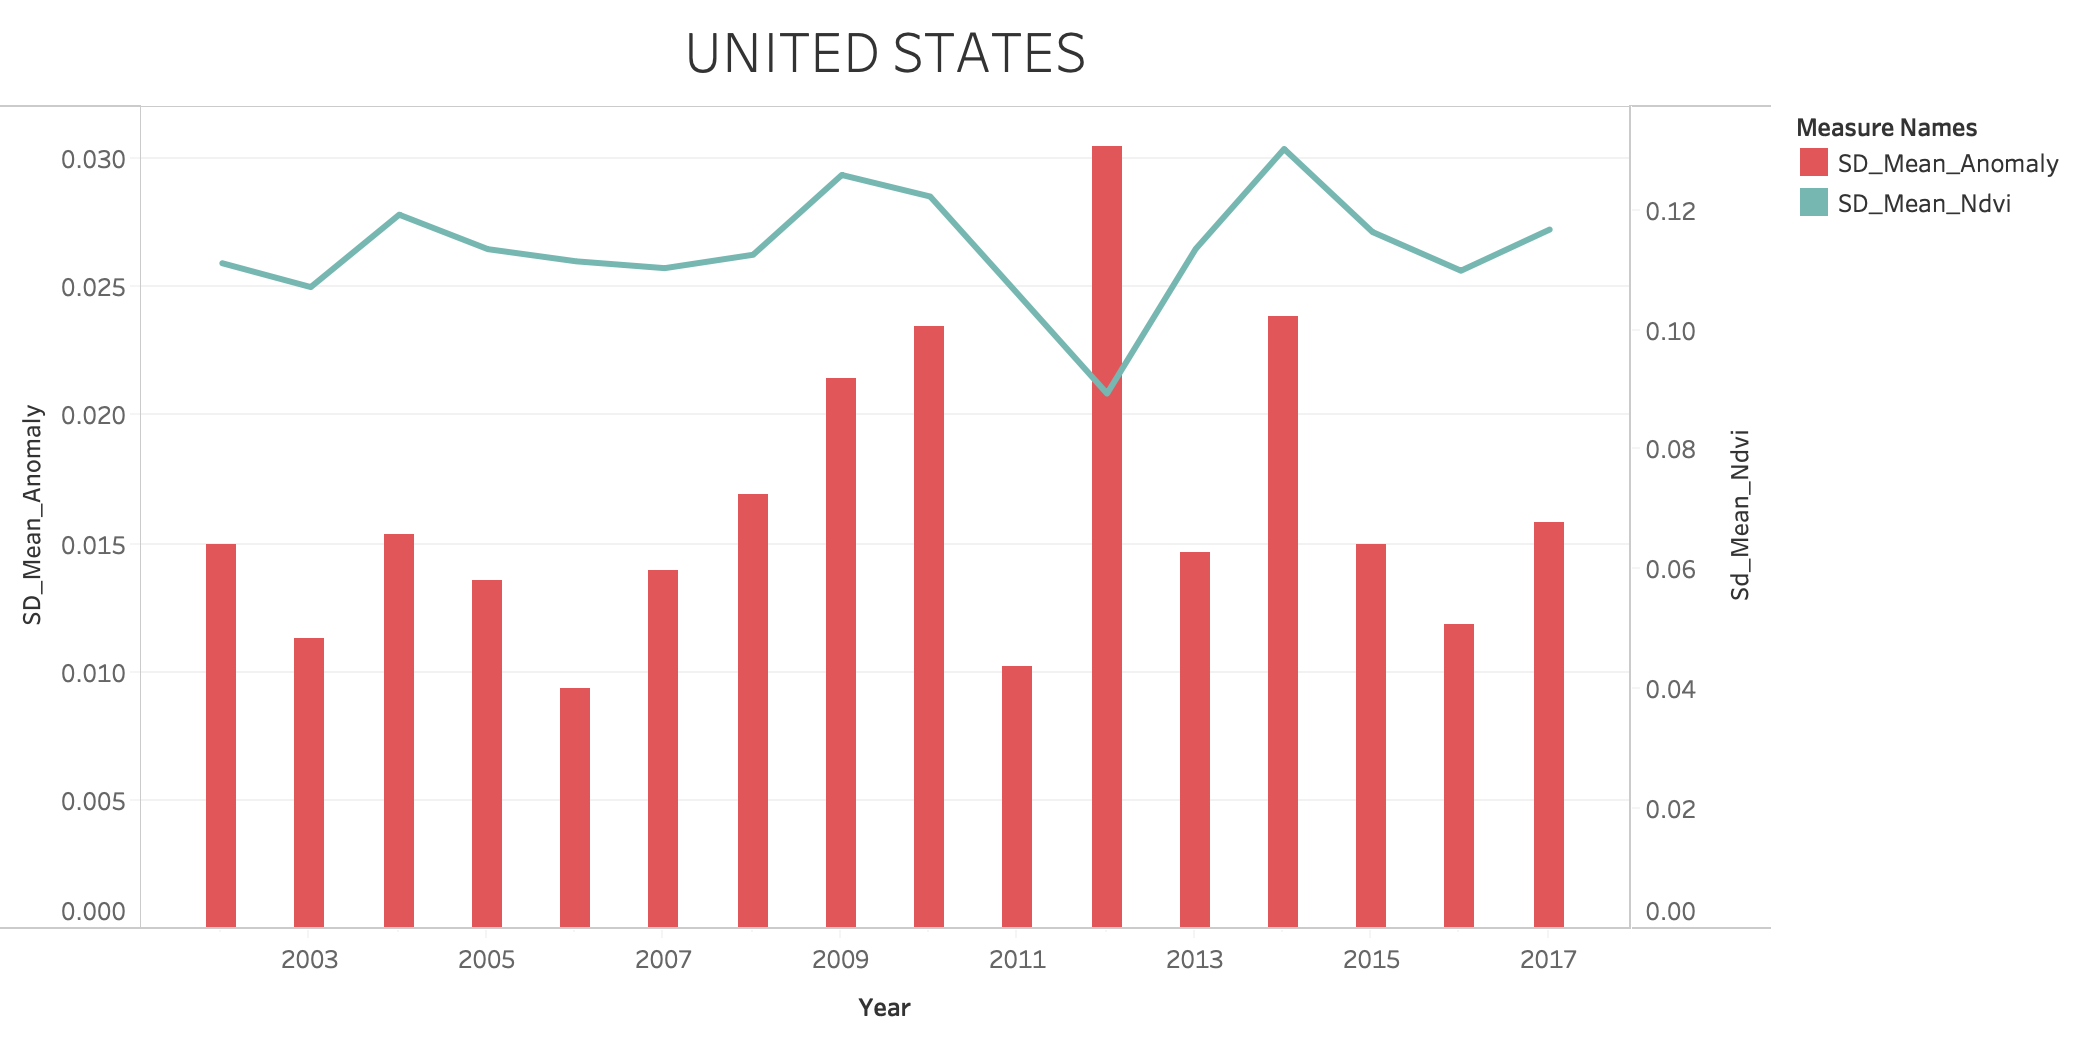
\includegraphics[width=0.5\linewidth]{figures/ch5/StandardDeviation/US_SD.png}
            \caption{\label{fig:US_SD}Standard deviation graph - United States}
    \end{figure}
    
    \clearpage
    \newpage

    
    \item \textbf{Histogram NDVI \& Anomaly distribution over the years}

    \begin{figure}[!htb]
        \begin{minipage}{0.5\textwidth}
            \centering
            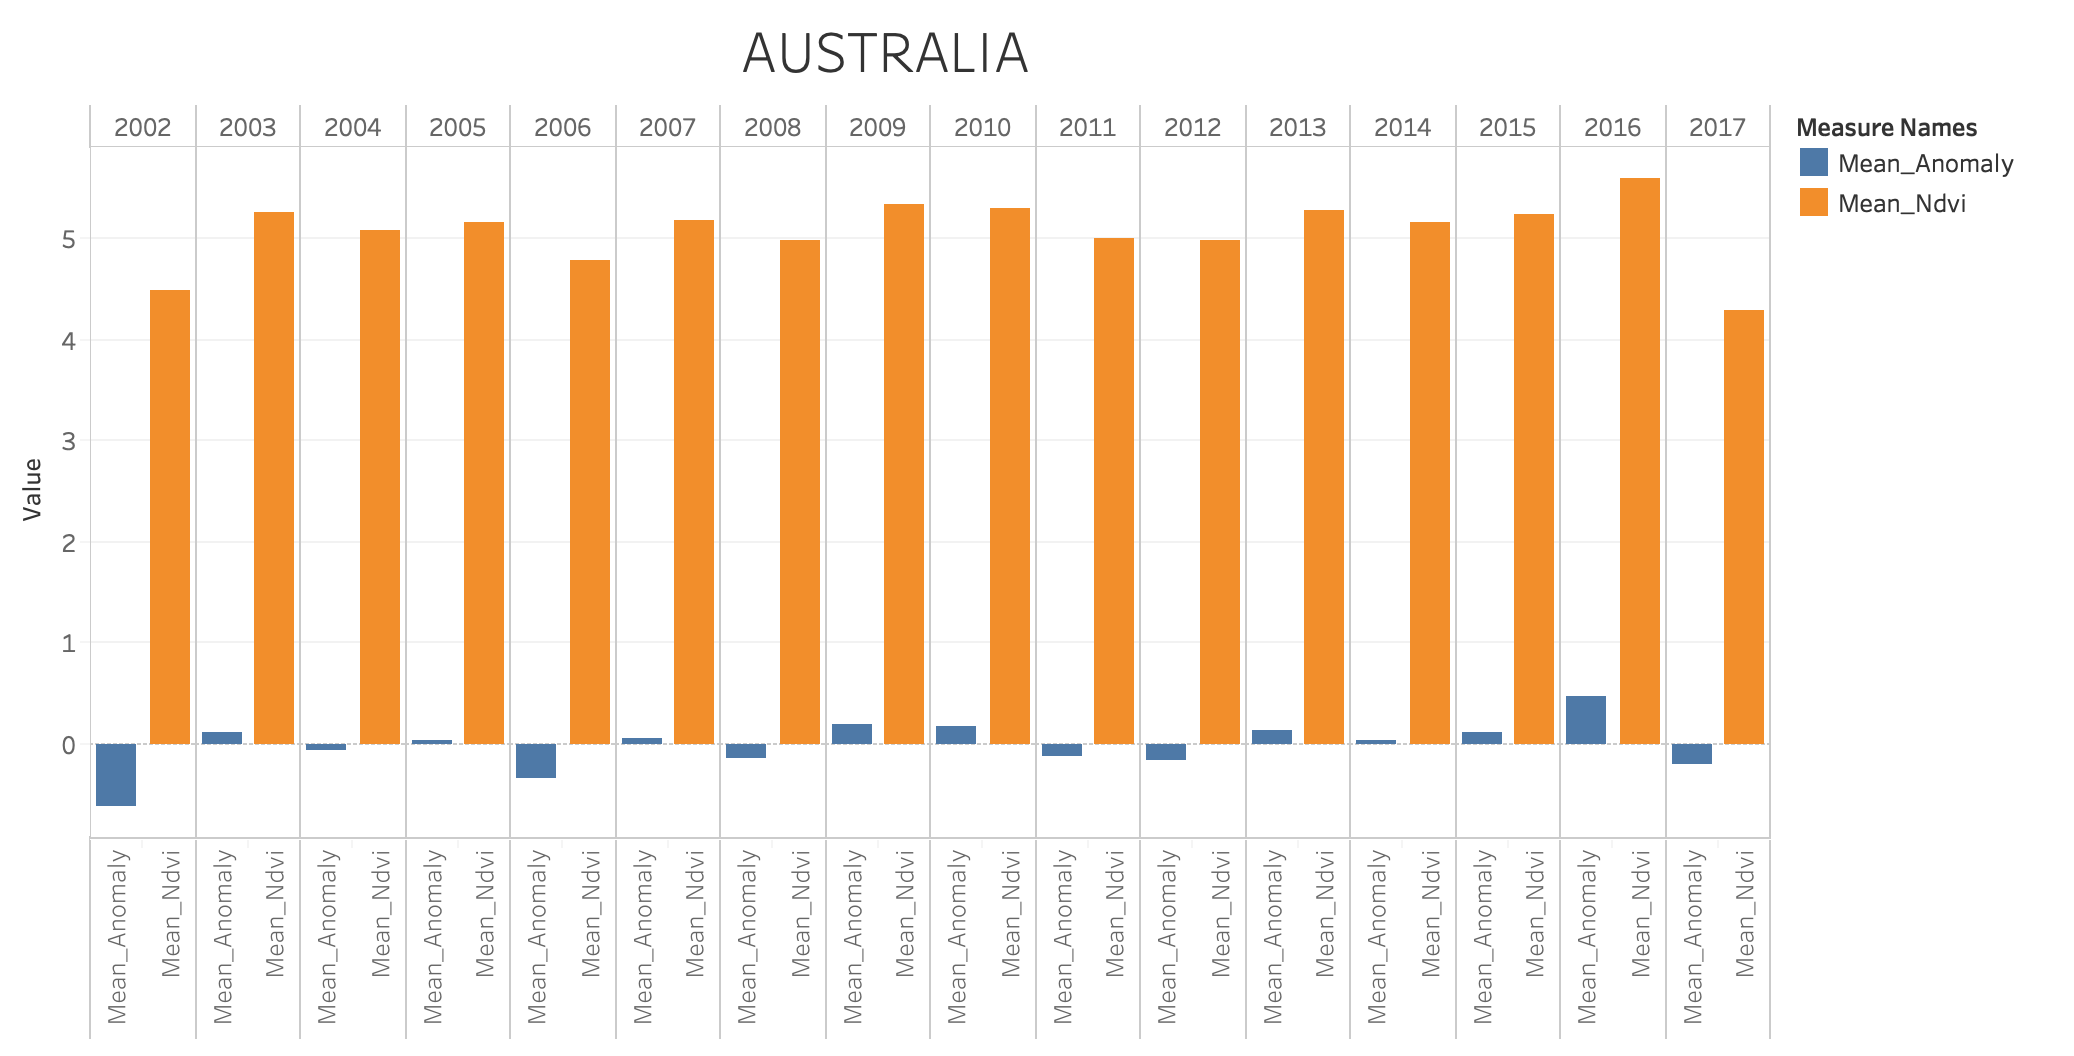
\includegraphics[width=1.0\linewidth]{figures/ch5/Histograms/AUSTRALIA_histogram.png}
            \caption{Histogram graph - Australia}\label{Fig:AUSTRALIA_histogram}
        \end{minipage}\hfill
        \begin{minipage}{0.5\textwidth}
            \centering
            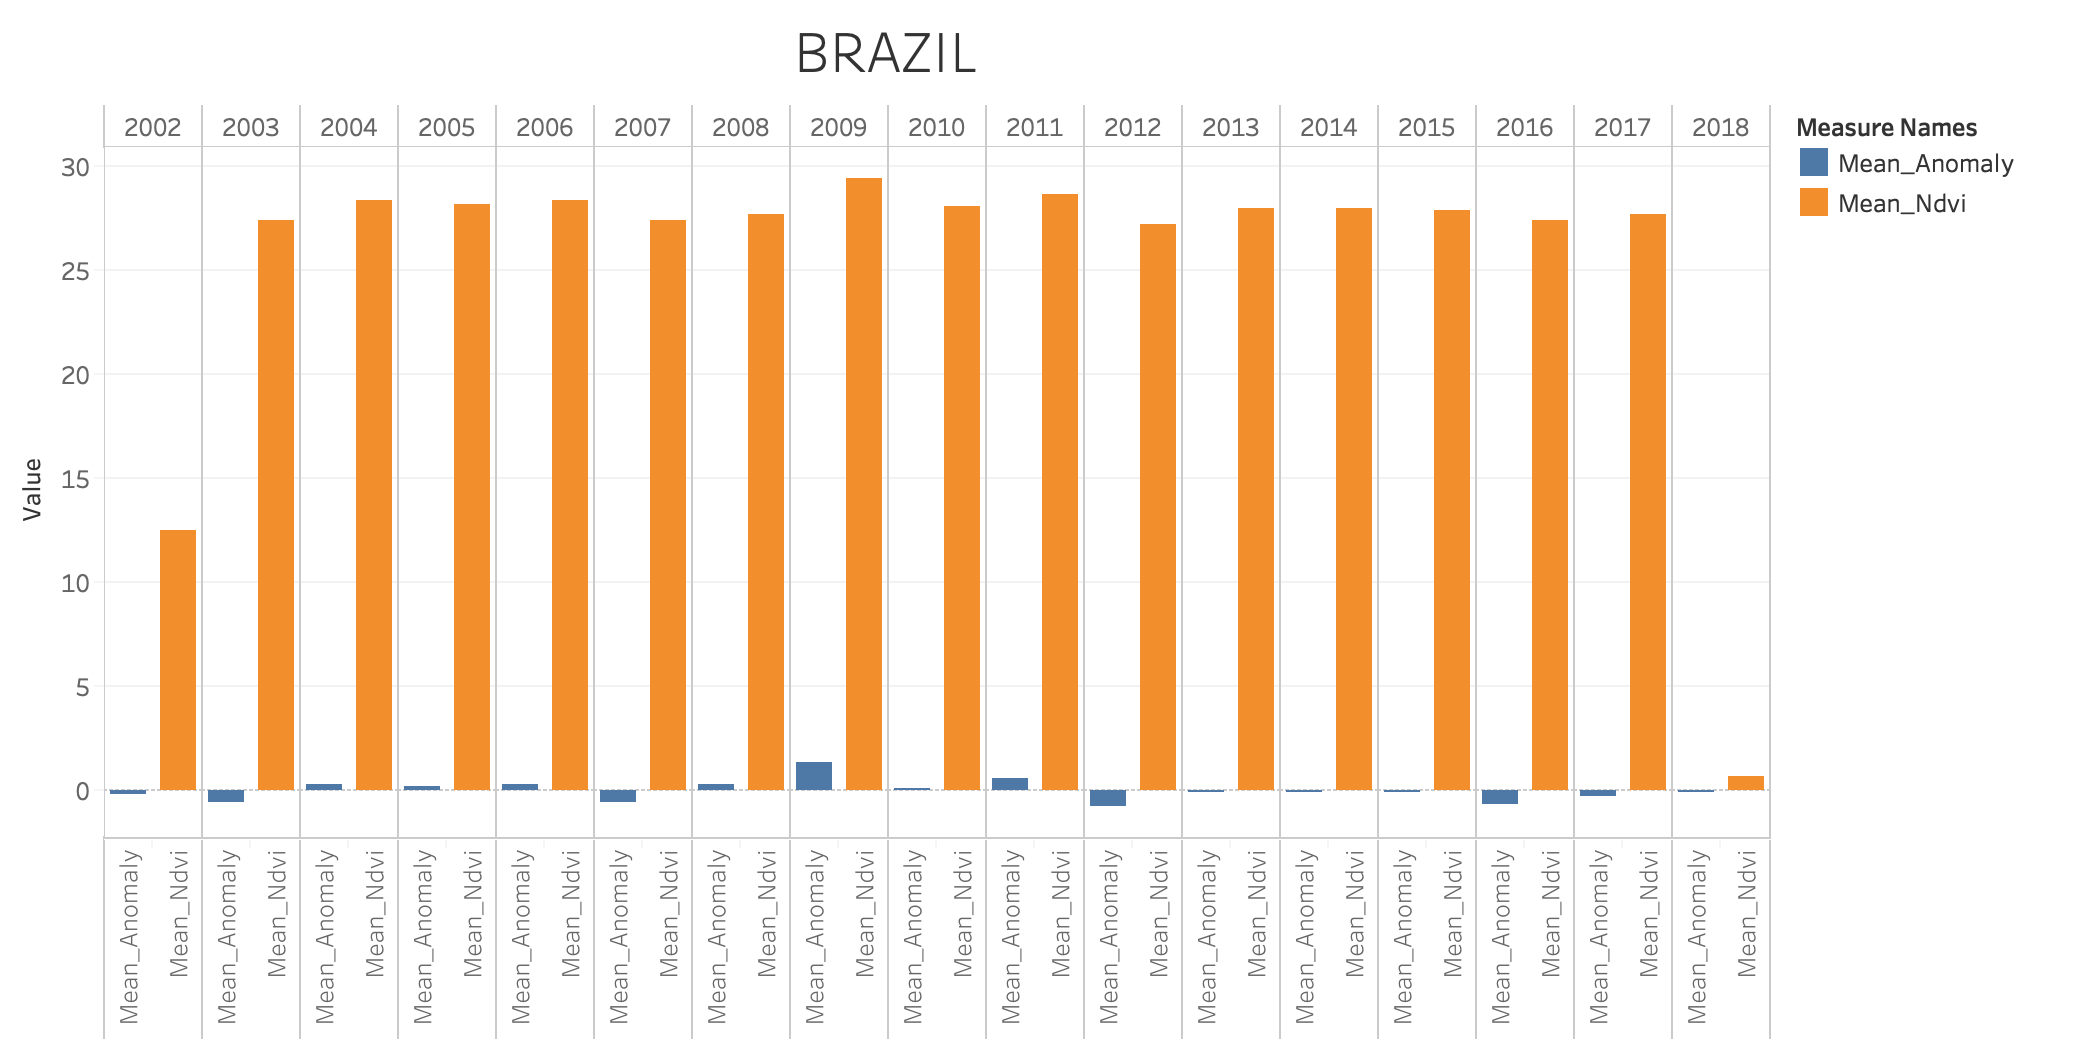
\includegraphics[width=1.0\linewidth]{figures/ch5/Histograms/BRAZIL_histogram.png}
            \caption{Histogram graph - Brazil}\label{Fig:BRAZIL_histogram}
        \end{minipage}
    \end{figure}
    
     \begin{figure}[!htb]
        \begin{minipage}{0.5\textwidth}
            \centering
            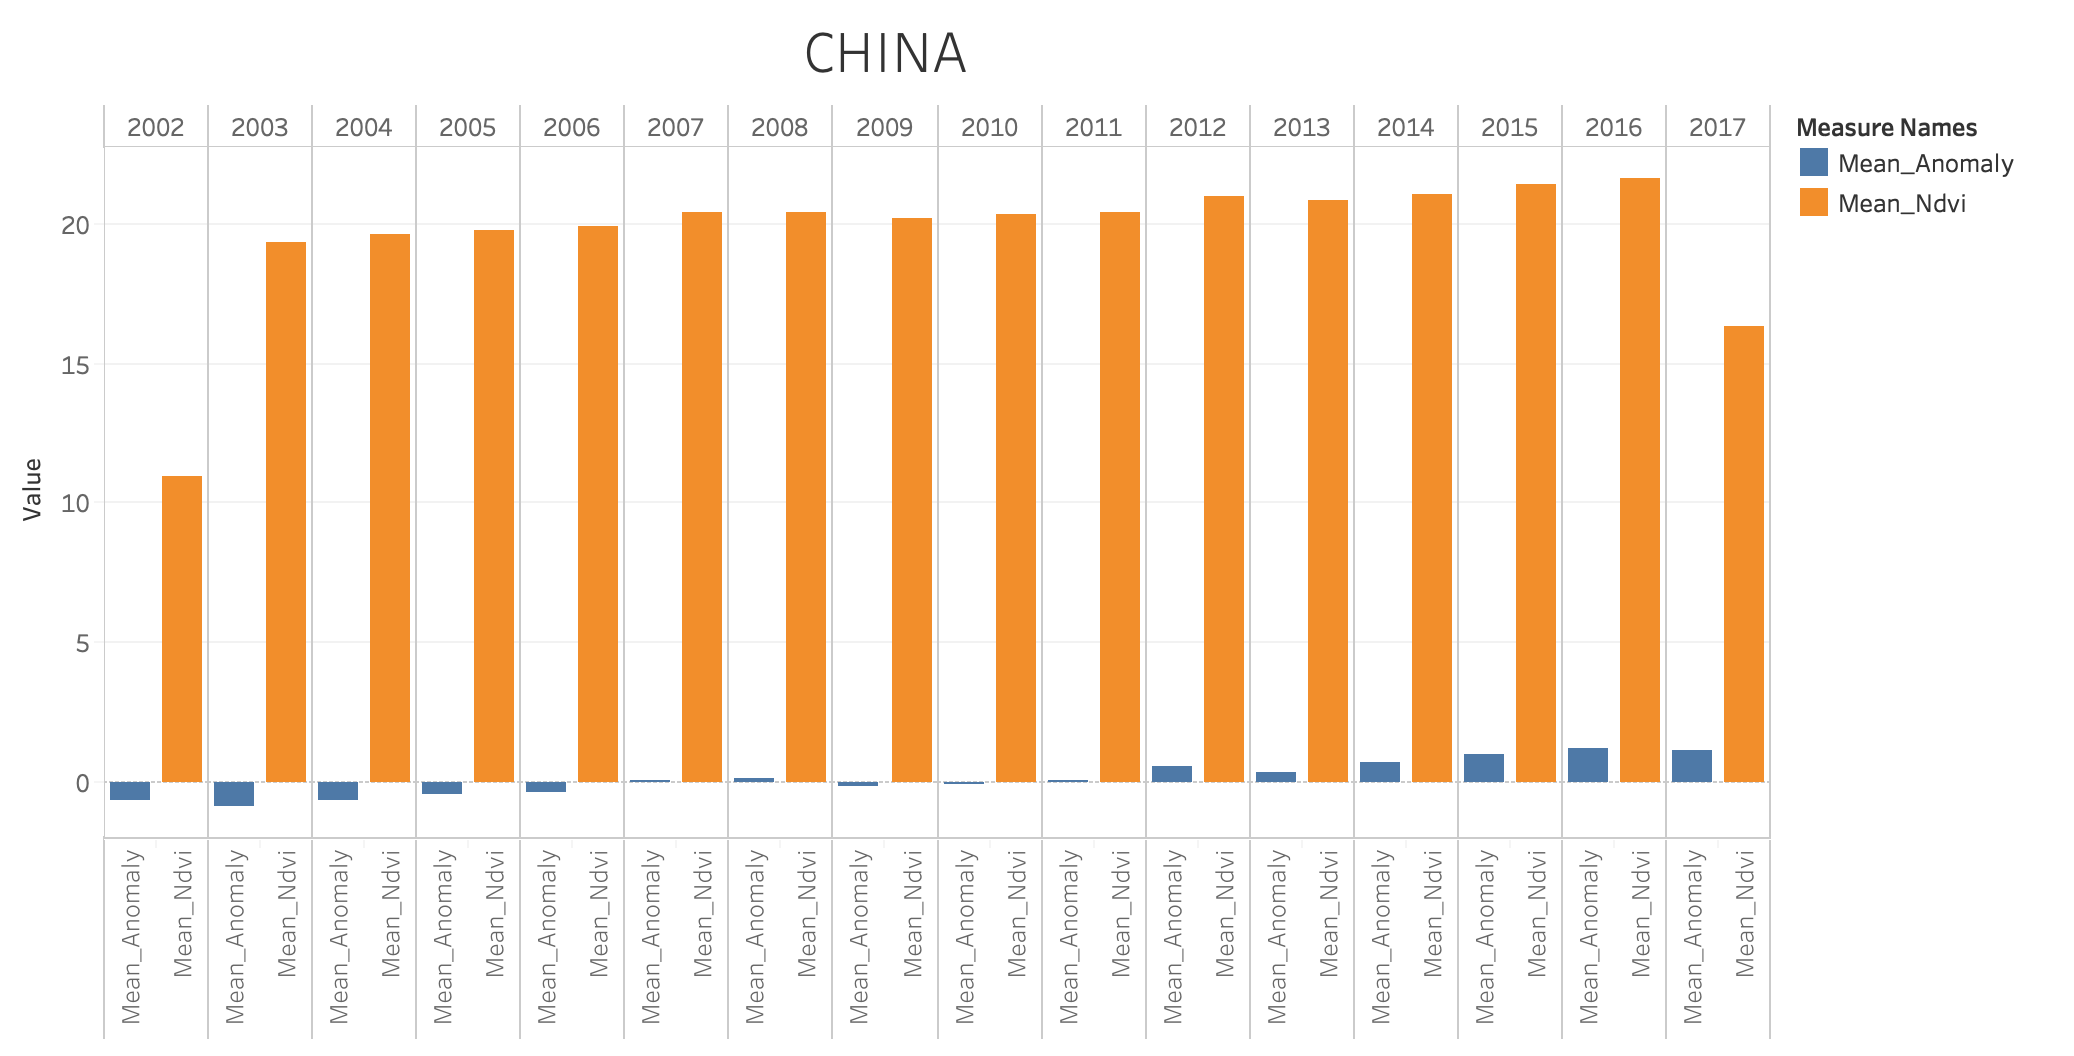
\includegraphics[width=1.0\linewidth]{figures/ch5/Histograms/CHINA_histogram.png}
            \caption{Histogram graph - China}\label{Fig:CHINA_histogram}
        \end{minipage}\hfill
        \begin{minipage}{0.5\textwidth}
            \centering
            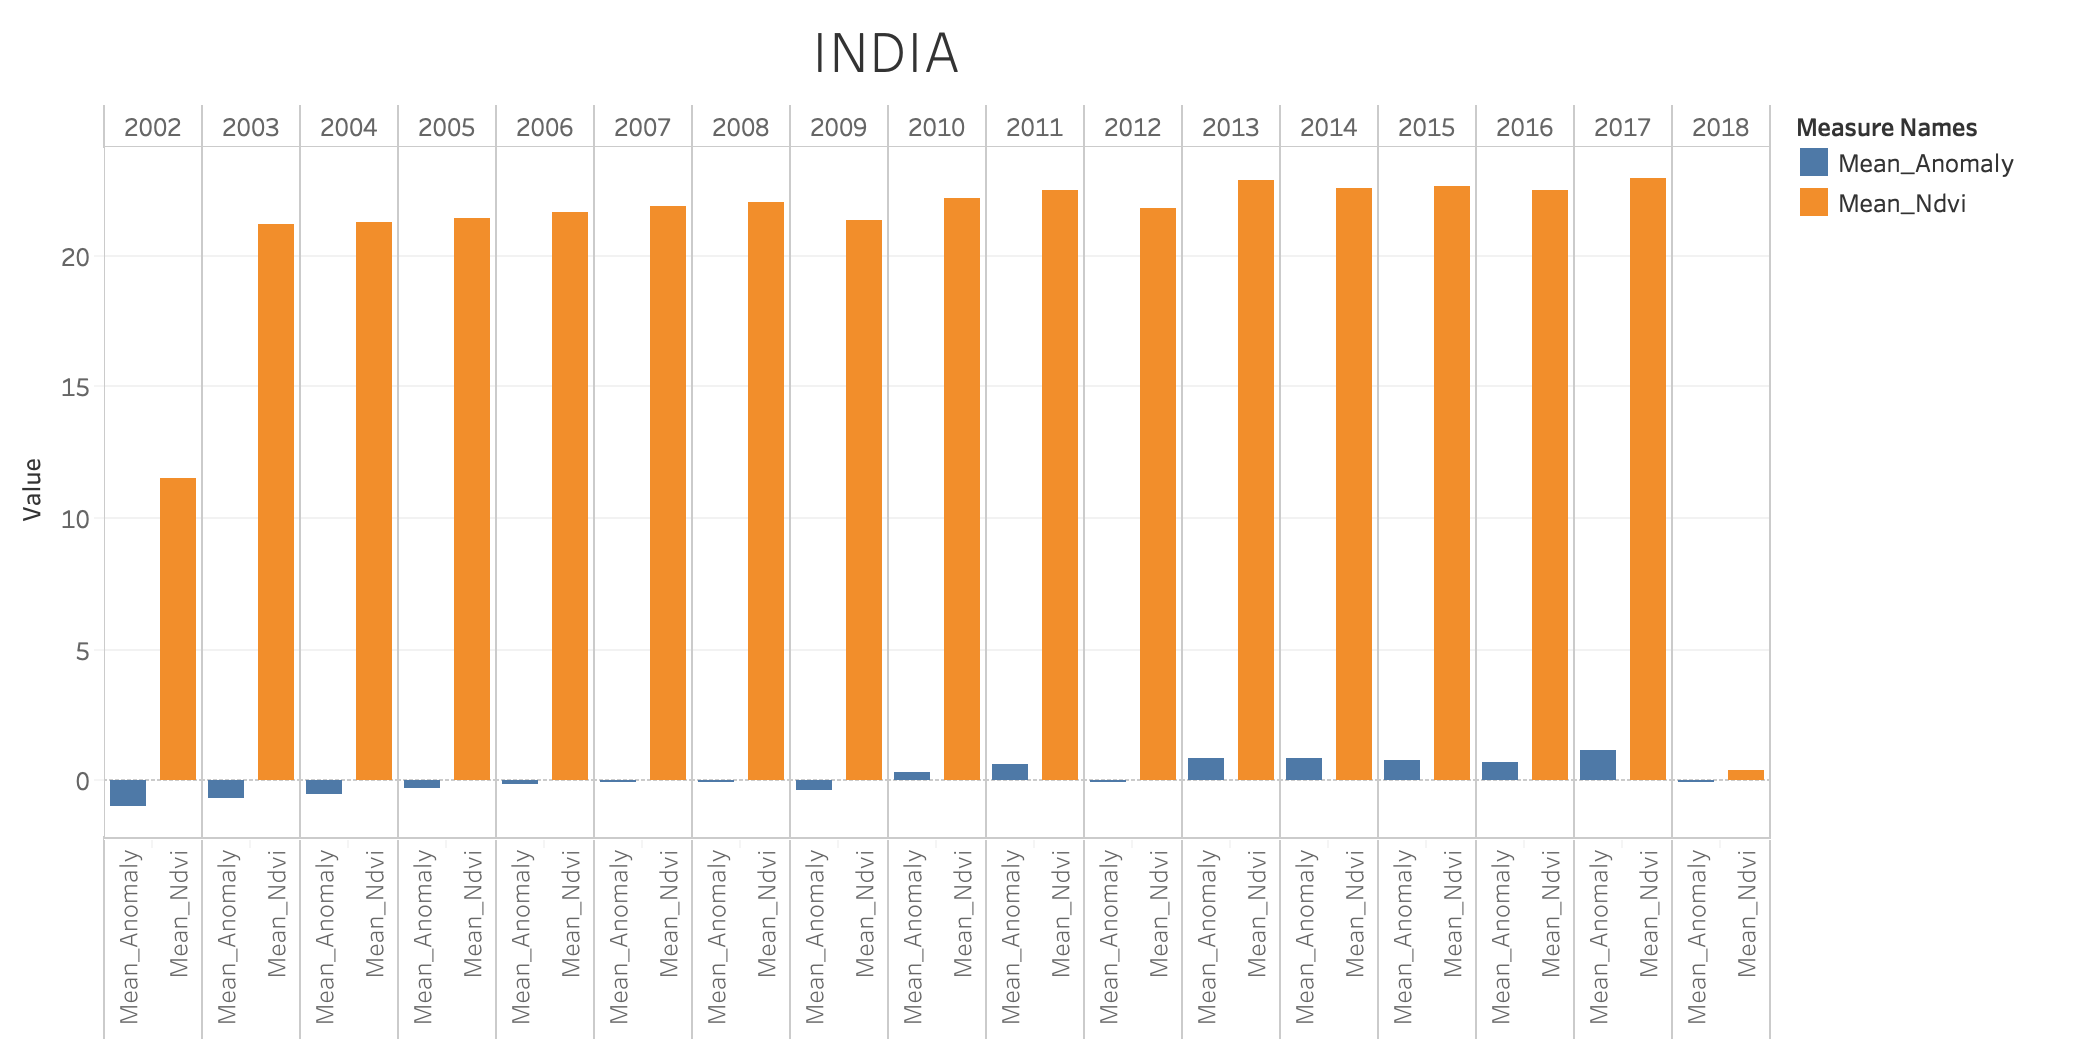
\includegraphics[width=1.0\linewidth]{figures/ch5/Histograms/INDIA_histogram.png}
            \caption{Histogram graph - India}\label{Fig:INDIA_histogram}
        \end{minipage}
    \end{figure}
    
     \begin{figure}[H]
            \centering
            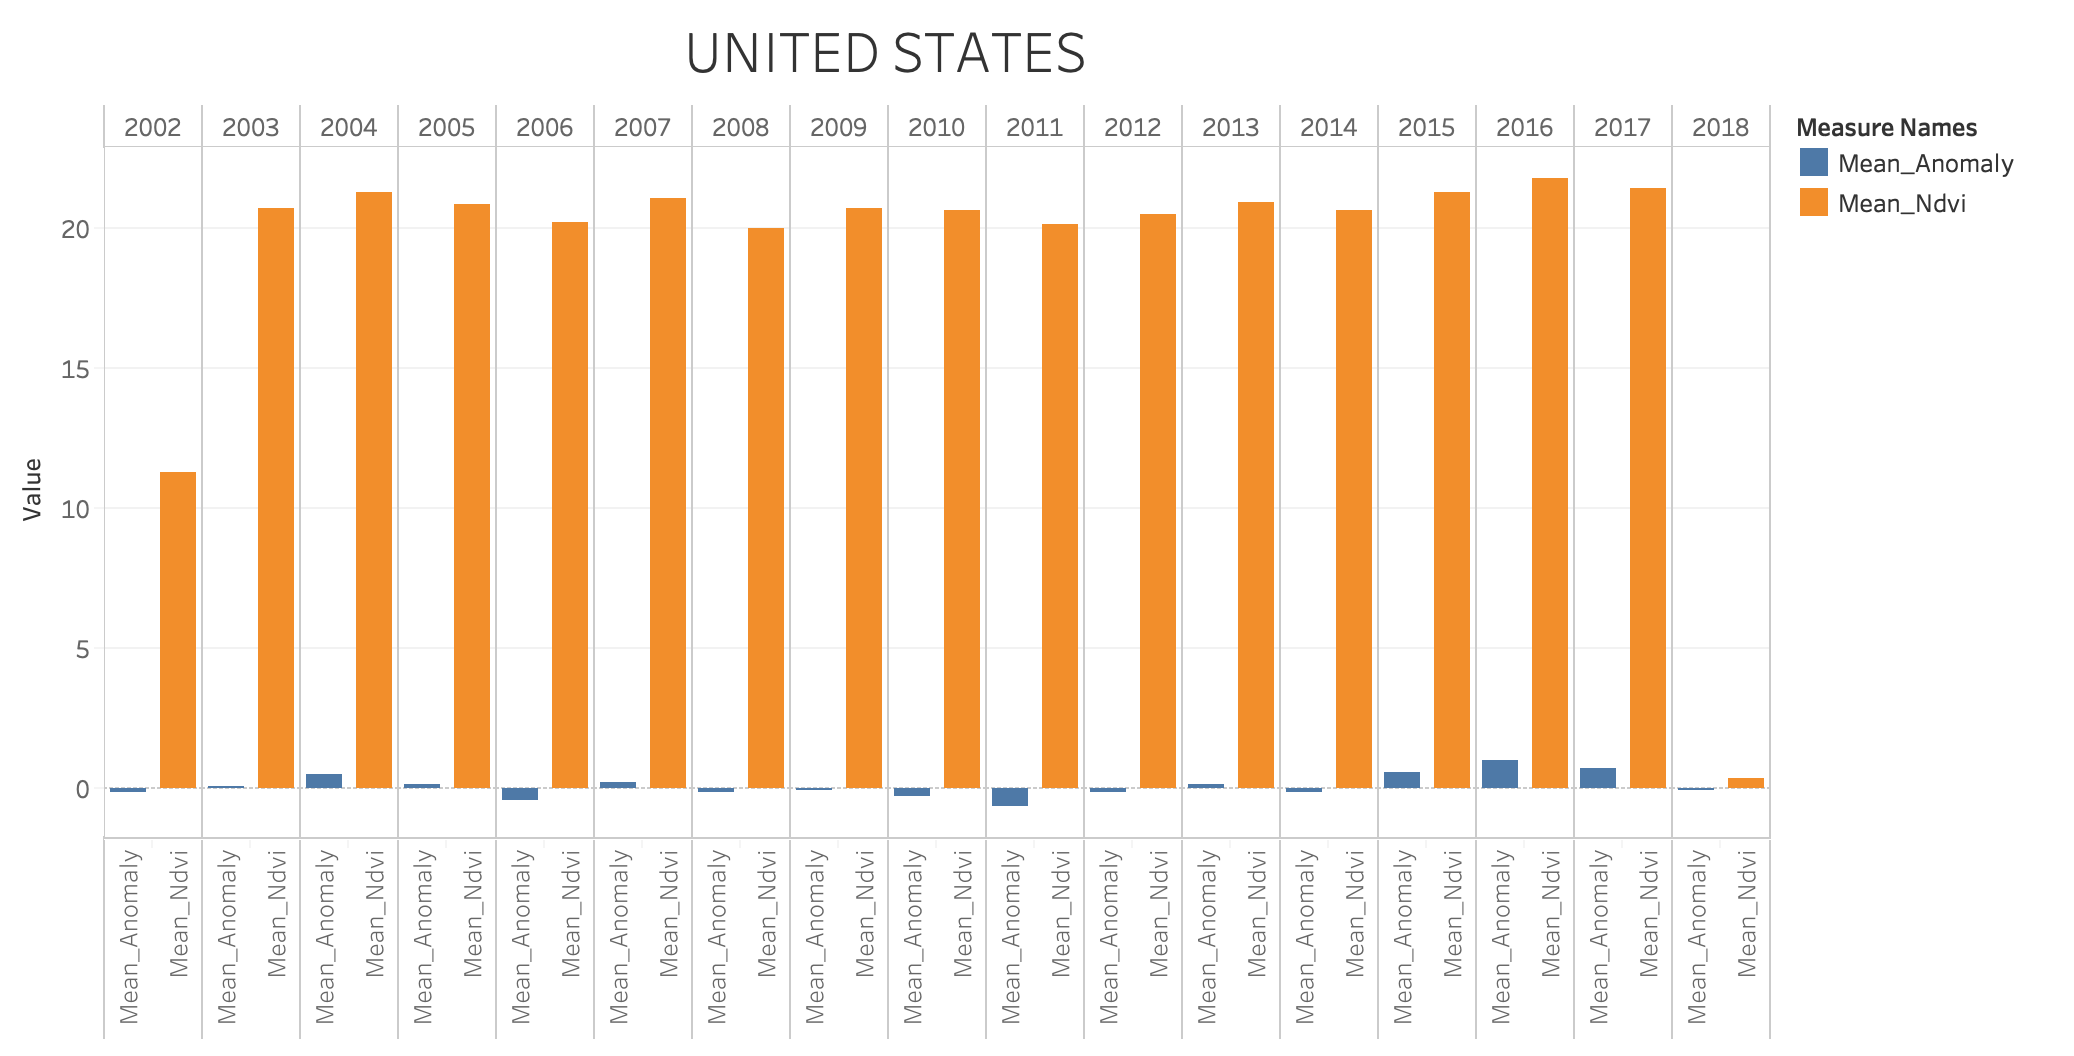
\includegraphics[width=0.5\linewidth]{figures/ch5/Histograms/US_histogram.png}
            \caption{\label{fig:US_histogram} Histogram graph - United States}
    \end{figure}
\newpage

\end{itemize}



